
\chapter{Modelling transit vehicles}
\label{cha:vehicle_model}

As vehicles travel along their respective routes, they report---in real-time---their geo\-graphical position as \gls{gps} coordinates. While these observations of location can be useful on their own, they also allow the inference of \emph{vehicle speed} which we cannot observe directly.\footnote{At least, not without being on the bus or standing on the roadside with a speed radar.} These speeds can then be mapped to physical road segments and used (in \cref{cha:network_model}) to update the network state.

Transit vehicles come in a variety of forms such as trains, trams, and buses. The last of these is the most notable for us since they are most affected by external factors, such as traffic congestion, and are therefore harder to predict. It is for this reason that we have used buses to develop the model presented in this chapter, which explores the following behaviours:
\begin{itemize}
\item general travel along a known path (including acceleration and deceleration);
\item bus stops, at which the bus may (or may not) stop;
\item intersections (both controlled and uncontrolled) which may (or may not) temporarily halt a bus; and
\item driver behaviour (this mostly comes under vehicle speed but is more significant in modelling buses versus trains).
\end{itemize}


\begin{knitrout}\small
\definecolor{shadecolor}{rgb}{0.969, 0.969, 0.969}\color{fgcolor}\begin{figure}

{\centering 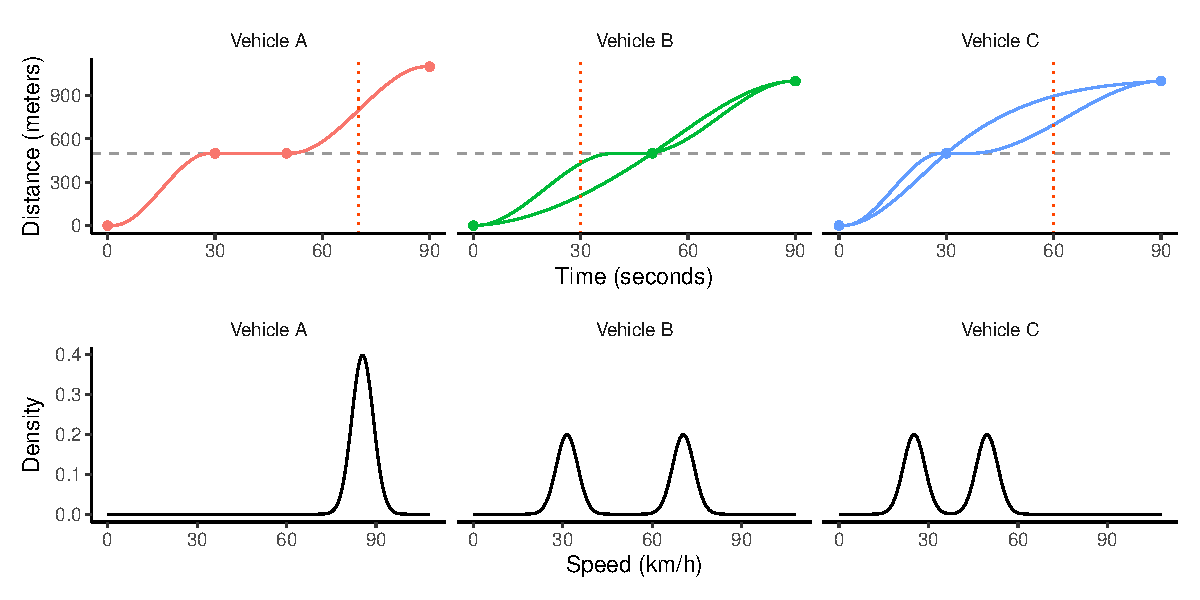
\includegraphics[width=\textwidth]{figure/vobs_multimode-1} 

}

\caption[Demonstration of multimodality in vehicle state]{Uncertainty in whether or not a bus stops can lead to multimodality in its speed dsitribution. Top: observations (points) with possible trajectories which fit the data. The horizontal dashed line represents the location of the stop, and the vertical dotted line indicates the time point at which we wish to estimate vehicle speed. Bottom: estimated speed distribution at the indicated time (dotted vertical line top graph).}\label{fig:vobs_multimode}
\end{figure}


\end{knitrout}


It is evident from the behaviours listed above (described in further detail in \cref{sec:vehicle_model}) that there are many factors involved in determining a bus's trajectory. Many of these factors, such as speed, are unmeasurable (but can be estimated), while others are often completely unknowable. An example of the latter is whether the bus stops at a bus stop. \Cref{fig:vobs_multimode} shows a series of \emph{distance} observations for three buses passing a stop:
\begin{itemize}
\item bus A stops and reports both its arrival and departure times;
\item bus B stops, but only reports its departure time;\footnote{This can happen if the arrival observation is ``lost'' or overwritten by the departure time within the \gls{gtfs} update interval.}
\item bus C does not stop and reports a departure time as it passes the stop.
\end{itemize}
Overlaid are possible trajectories for each vehicle: for bus A, there is only one since we observe both the vehicle's arrival and departure. However, B and C each have two potential paths: one in which the vehicle stops, and another in which it does not. The main point is that \emph{we cannot know which is true}, leading to \emph{multimodality} in the vehicle's state. In the lower half of \cref{fig:vobs_multimode} are the possible distributions of the vehicles' speeds at the time marked with a dotted vertical line above. For bus A, the distribution is \emph{unimodal}, which satisfies the assumptions of many estimation methods (such as the Kalman filter, \cref{sec:kf}). For buses B and C, however, the speed state is \emph{bimodal}, so the Kalman filter would no longer be an appropriate choice for these data. This multimodality was one of the main reasons we chose to use a particle filter to implement the vehicle model, as it does not encounter these same issues and is ideal for sampling a wide range of trajectories \citep{Hans_2015}.

Once the vehicle's state has been estimated, we can make inferences about its average speed along a given road segment, which we cover in \cref{sec:vehicle_speeds}. This includes a simulation comparing the models introduced in \cref{sec:vehicle_model}, and showing the effectiveness of our approach with simulated data. I conclude this chapter with a discussion of the real-time implementation of the model (\cref{sec:particle-filter}), including the process of parameter estimation for the various model parameters, and details of some difficulties experienced while modelling these data.



\section{Real-time estimation of vehicle state}
\label{sec:vehicle_model}

Real-time vehicle tracking has been the centre of much research, particularly for robotics applications and self-driving cars \citep{Daum_2005, Gustafsson_2002}. In many of these, data is sampled at a very high frequency, often multiple times per second, leading to high-accuracy estimates of the object's \emph{state}. Alas, with transit data this is seldom the case; instead, it is common for observations to be reported once every 10--30 seconds or, in some cases, even longer.

Low-frequency observations lead to high uncertainties of state parameters and difficulty capturing all possible trajectories, which can lead to degradation of the model and loss of information. In \cref{fig:vobs_multimode}, we show two possible trajectories for buses B and C; there are, in fact, countless possibilities: perhaps the bus waited at the stop a little longer? In this case, there is uncertainty about the bus's dwell time and speed; however, the first step of \agls{rbm} is to \emph{predict} the upcoming state \emph{before observing it} (\cref{sec:recursive-bayes}). If the model does not cover the vehicle's actual trajectory, we effectively ``lose'' the vehicle, and the filter is said to \emph{degenerate} \citep{Chen_2014}. In that case, we typically need to reinitialise the vehicle's state, resulting in a loss of any information we might have gained in the last time step.

When deciding which type of model implementation to use, historically the most common for this type of data is the Kalman filter \citep{Wall_1999, Dailey_2001, Cathey_2003}. However, it assumes a Gaussian state distribution, which I have demonstrated is not the case. Instead, we use a \emph{particle filter} due to its high flexibility and ability to explore a broad set of plausible trajectories \citep{Hans_2015} and excels in situations where there are multiple distinct possiblities, as in \cref{fig:vobs_multimode} \citep{Ulmke_2006}. This makes it well suited for transit modelling, and has been used in many other vehicle tracking applications \citep{Davidson_2011,Gustafsson_2002,Gustafsson_2010,Ulmke_2006}.

\begin{knitrout}\small
\definecolor{shadecolor}{rgb}{0.969, 0.969, 0.969}\color{fgcolor}\begin{figure}

{\centering 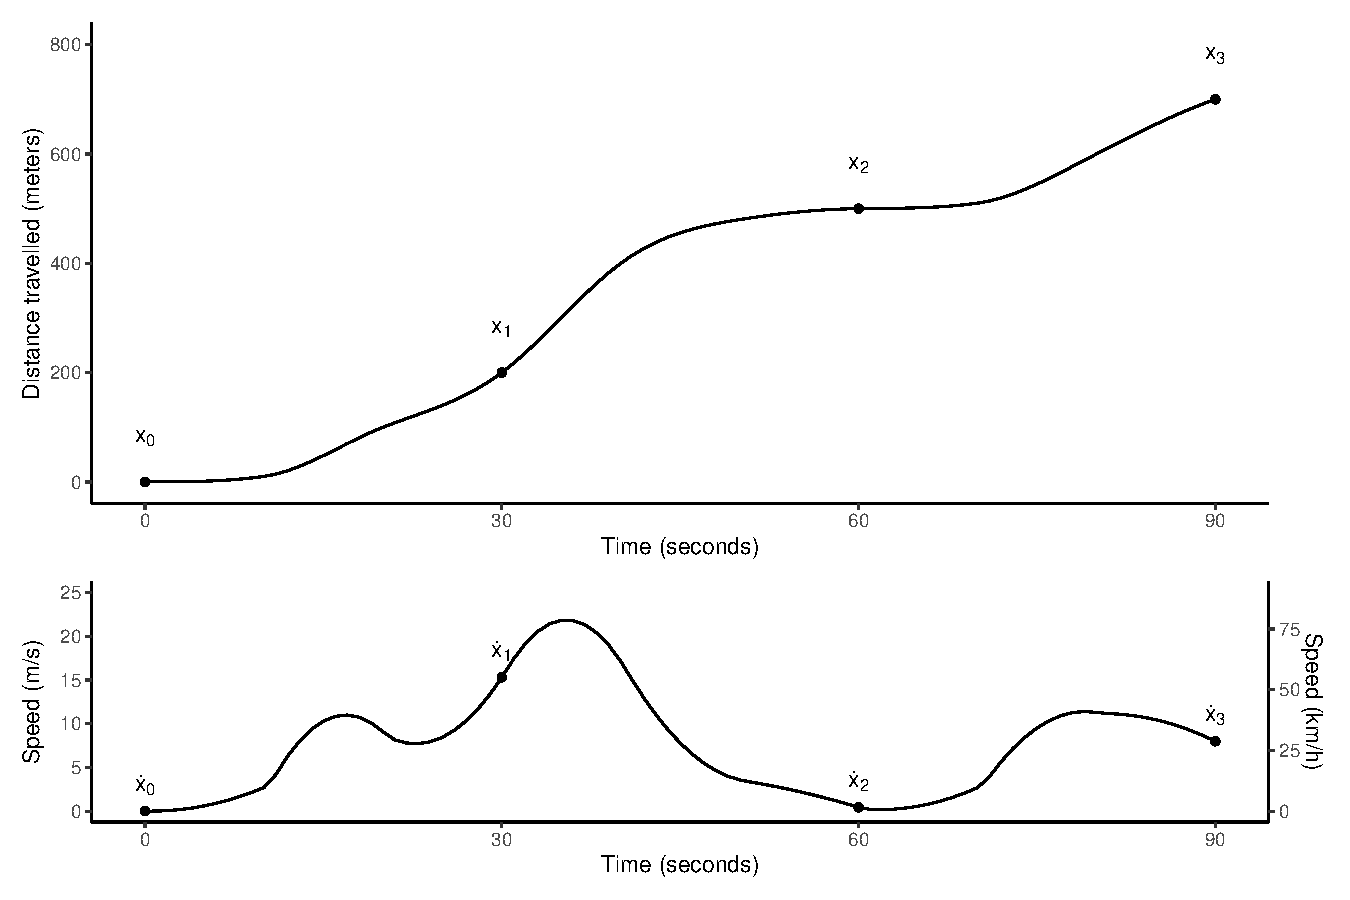
\includegraphics[width=\textwidth]{figure/vehicle_state-1} 

}

\caption[Visualisation of vehicle state showing \emph{distance travelled} and \emph{speed}]{Visualisation of vehicle state showing \emph{distance travelled} and \emph{speed}. The distance travelled, $x$, over time includes points of observed states $\Vstate_k, k=0,\ldots,3$. The gradient of distance over time is speed, $\dot x$: steeper sections of the top graph correspond to higher speeds, and vice verca. The speed graph also includes a second right-hand axis with speed in kilometers per hour (km/h) for reference.}\label{fig:vehicle_state}
\end{figure}


\end{knitrout}

The vehicle model itself involves describing bus behaviour algorithmically to infer the vehicle's \emph{unknown state} $\Vstate_k$ from a sequence of \gls{gps} observations. Since buses service routes with a known path, we represent their position using \emph{distance travelled} along the route's path, which we denote $\Vdist_k$ at time $\Vtime_k$. Additionally, we are interested in the \emph{speed} of the vehicle, $\Vspeed_k$. Therefore, the underlying, unknown, and \emph{unobservable} state of a vehicle at time t is denoted
\begin{equation}
\label{eq:vehicle_state}
\Vstate_k = \tvec{\Vdist_k, \Vspeed_k}.
\end{equation}
\Cref{fig:vehicle_state} graphs a series of vehicle states with time along the x-axis and distance travelled (in meters) along the y-axis. The derivative (gradient) of the curve represents the vehicle's speed. So, for example, the vehicle state at time $t_1 = 30$~seconds is $\Vstate_1 = [\Vdist_1, \Vspeed_1]^\top = [200~\text{m}, 15~\text{m/s}]^\top$. The remainder of this section presents a model, along with a particle filter implementation of it, to estimate vehicle state.

The particle filter represents the vehicle's state using a sample of \emph{particles}, each with an individual state, $\Vstate_k\vi$. We can think of each particle as an ``imaginary bus'' which represents one possible state (and associated trajectory) of the true bus. Together, the particles approximate the posterior distribution of the vehicle's state at time $\Vtime_k$ given all observations up to time $\Vtime_k$, denoted $\Vobs_{1:k}$. The posterior distribution is expressed using the Dirac delta measure, $\dirac$, (\cref{app:dirac-delta-measure}):
\begin{equation}
\label{eq:vehicle_state_dirac}
p(\Vstate_k \cond{} \Vobs_{1:k}) \approx
\sum_{i=1}^\Np \Pwt_{k-1} \dirac_{\Vstate_k\vi}\left(\Vstate_k\right).
\end{equation}

Before implementing \agls{rbm} for these data, we need a \emph{transition function}, a \emph{measurement function}, and a \emph{likelihood}. The transition function, $\Vtrans$, describes how a vehicle behaves between two consecutive observations: that is, the shape of the curves in \cref{fig:vehicle_state}. This allows us to \emph{predict} the future state of the vehicle \emph{given its last known state}. Additionally, we include the \emph{system noise} parameter $\Vnoise$~m/s$^2$, which represents the rate of change of speed. The measurement function, $\Vmeas$, describes the relationship between the vehicle's state, $\Vstate_k$, and the observation of this state, $\Vobs_k$, which is a \gls{gps} location with an associated \emph{measurement error}, $\GPSerr$. We represent this using two simple equations,
\begin{equation}
\label{eq:vehicle_model}
\begin{split}
\Vstate_k &= \Vtrans(\Vstate_{k-1}, \Vnoise), \\
\Vobs_k &= \Vmeas(\Vstate_k) + \GPSerr.
\end{split}
\end{equation}
The \emph{likelihood} function quantifies the plausibility of an observation $\Vobs_k$ given an underlying state $\Vstate_k$.


We now discuss the details of the two components of the model and their implementations. The \emph{prediction step} (\cref{sec:vehicle_model_trans}) supplies an estimate of the bus's state \emph{before observing it} by using a model of bus behaviour. Then the \emph{update state} (\cref{sec:pf-likelihood}) combines the prediction and observation, using the measurement function and likelihood, to obtain a posterior estimate of the vehicle's state.

\subsection{Predicting vehicle state: the transition function}
\label{sec:vehicle_model_trans}

The aim of the prediction step is to obtain a \emph{prior predictive distribution} of the vehicle's state at time $\Vtime_k$ based on its previous state at time $\Vtime_{k-1}$, $p(\Vstate_k \cond{} \Vstate_{k-1})$. Using the model definition in \cref{eq:vehicle_model} along with the particle filter approximation of state in \cref{eq:vehicle_state_dirac}, we can write the prior prediction of the vehicle's state as
\begin{equation}
\label{eq:vehicle_pf_predict}
p(\Vstate_k \cond{} \Vstate_{k-1}) \approx
\sum_{i=1}^\Np
    \Pwt_{k-1}
    \DiracMeasure{\Vstate_k\vi}{\Vstate_k},
\end{equation}
where $\Vstate_k\vi = f(\Vstate\vi_{k-1}, \Vtdiff_k, \Vnoise)$ and $\Vtdiff_k = \Vtime_k - \Vtime_{k-1}$.

The transition function $\Vtrans$ is where we define the vehicle behaviours mentioned earlier. Kalman filter applications are limited to linear transformations of the state which can be expressed in a \emph{transition matrix}. However, \cref{eq:vehicle_pf_predict} shows that, in the case of the particle filter, the transition function is applied to each particle independently, allowing for a lot more flexibility in $\Vtrans$. We now describe the various model components of $\Vtrans$, implemented as an algorithm in the \pkg{transitr} package (see \cref{sec:particle-filter} for details). The core components are vehicle motion (speed and acceleration along a known path), stopping behaviour at known locations (bus stops and intersections), as well as the ability to handle several other scenarios to avoid degeneration.


\subsubsection{Component A: vehicle motion}
\label{sec:vehicle_model_behaviour}

The first behaviour to consider is the vehicle's motion along a known path: the \emph{speed} at which a vehicle is travelling will affect where it ends up. Since speed, $\Vspeed$, is the derivative of distance travelled over time, if $x = d(t)$, then $\Vspeed = d'(t)$, which is shown visually back in \cref{fig:vehicle_state}. It follows that we can predict a vehicle's future state, given its current state (distance travelled and speed) and system noise, $\Vnoise$, which is interpreted as \emph{the average change in speed per second}:
\begin{equation}
\label{eq:vehicle_model_newton}
\Vstate_{k|k-1} = f_{A1}\left(\Vstate_{k-1|k-1}, \Vtdiff_k, \Vnoise\right) =
\begin{bmatrix}
\Vdist_k \\ \Vspeed_k
\end{bmatrix} =
\begin{bmatrix}
\Vdist_{k-1} + \Vtdiff_k\Vspeed_k \\
\Vspeed_{k-1} + v_k
\end{bmatrix}
\end{equation}
where
\begin{equation}\label{eq:vehicle_model_newton_noise}
v_k \sim \TNormal{0}{\Vnoise}{-\Vspeed_{k-1}}{30 - \Vspeed_{k-1}}.
\end{equation}
The noise term is truncated to ensure the new speed is both positive and under 30~m/s, which is 108~km/h (the maximum road speed in Auckland is 100~km/h). The resulting transition function, $\Vtrans_{A1}$, is easily implemented by simulating, for each particle, a new speed before calculating the final state using \cref{eq:vehicle_model_newton}. A similar model was used by \citet{Cathey_2003,Dailey_2001}.


\Cref{fig:transition_demo} demonstrates transition model $\Vtrans_{A1}$ (left) using a sample of $N=10$~particles which, at time $t_{k-1}$, take one of three unique states (due to resampling in the previous iteration, \cref{sec:pf}). The points have been coloured by their initial state to demonstrate the effect of adding system noise \emph{before} transitioning to allow the particles to disperse. Not doing so would, in this instance, yield only three unique states in the final predictive distribution.

\begin{knitrout}\small
\definecolor{shadecolor}{rgb}{0.969, 0.969, 0.969}\color{fgcolor}\begin{figure}

{\centering 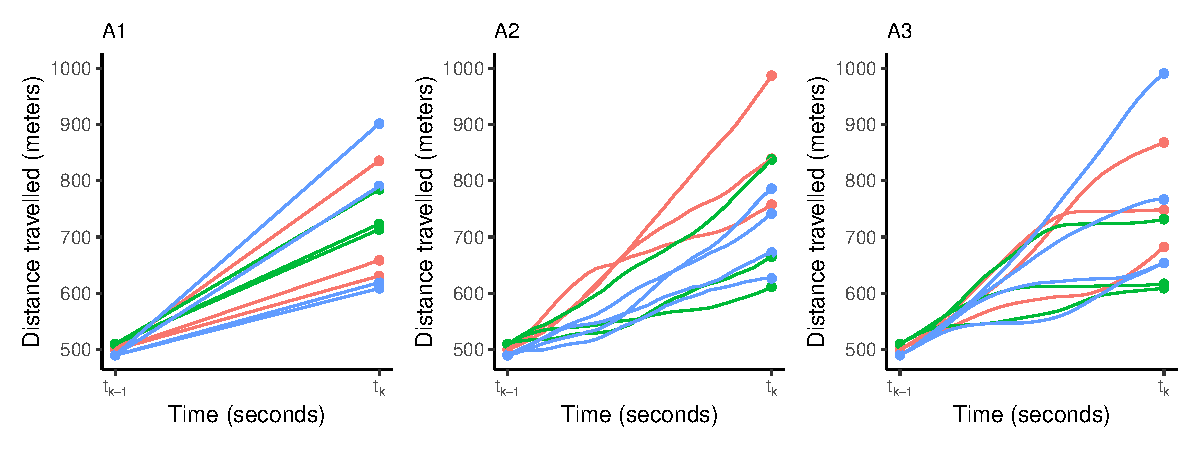
\includegraphics[width=\textwidth]{figure/transition_demo-1} 

}

\caption[Simulated particle trajectories using three transition functions]{Simulated particle trajectories using three transition functions, $f_{A1}$, $f_{A2}$, and $f_{A3}$ from left to right. Points have been coloured by their parent (after resampling) to demonstrate the affect of system noise.}\label{fig:transition_demo}
\end{figure}


\end{knitrout}

The main issue with this model is that it assumes constant speed between observations, which---given Auckland traffic---is unlikely to be the case. In \cref{fig:vehicle_state}, we showed speed varying over time, even between observations. To model this, we \emph{iteratively} update the vehicle's state\footnote{This is one advantage of the particle filter---we can easily perform iterative updates!} by reusing \cref{eq:vehicle_model_newton} $\Vtdiff_k$ times, setting $\Vtdiff_k=1$ in each iteration. The second graph in \cref{fig:transition_demo} shows the effect this has on the particles' trajectories.


Of course, if speed is the first derivative of the vehicle's trajectory function, then \emph{acceleration} is the second, $\Vaccel = d''(t)$. In this case, we add a third component to the vehicle's state and consider speed similarly to distance. The transition function
\begin{equation}
\label{eq:vehicle_model_newton_accel}
\Vstate_{k|k-1} = \Vtrans_{A3}\left(\Vstate_{k-1|k-1},\Vtdiff_k,\Vnoise\right)
\end{equation}
is iterative. It is initialised with $\bz_0 = \Vstate_{k-1|k-1}$ and repeated for $s = 1, \ldots, \Vtdiff_k$ to obtain $\Vstate_{k|k-1} = \bz_{\Vtdiff_k}$:
\begin{equation}
\label{eq:vehicle_model_newton_accel_iter}
\bz_s =
\begin{bmatrix}
z_s \\ z_s \\ z_s
\end{bmatrix} =
\begin{bmatrix}
z_{s-1} + \dot z_s \\
\dot z_{s-1} + \ddot z_s \\
\ddot z_{s-1} + v_s
\end{bmatrix}.
\end{equation}
System noise (interpreted as \emph{the average change in acceleration per second}) is applied to the acceleration term and truncated to ensure the speed remains positive and less than 30~m/s,
\begin{equation}
\label{eq:vehicle_model_accel_dist}
v_s \sim \TNormal{0}{\Vnoise}{-\dot z_{s-1} - \ddot z_{s-1}}{30 - \dot z_{s-1} - \ddot z_{s-1}}.
\end{equation}
These trajectories are shown in the third graph of \cref{fig:transition_demo}. The main issue with $\Vtrans_{A3}$ is that it is difficult to parameterize and constrain the acceleration to ensure speed remains within the interval $(0,30)$ while preserving the function's ability to generate plausible trajectories.



\subsubsection{Component B: stopping at nodes}
\label{sec:vehicle_model_nodes}

In \cref{sec:route-segments}, we discussed using a road network consisting of nodes---either bus stops or intersections---and the roads connecting them. This \emph{segmentisation} allows each route to be expressed as a \emph{sequence of nodes} and connecting \emph{road segments}. Component A of the transition model deals with vehicle behaviour along the road segments; we now examine bus behaviour at nodes.

There are two types of nodes in our framework: \emph{bus stops} where passengers can board and disembark, and \emph{intersections} where buses (and other road users) wait depending on congestion levels and traffic lights. In each case, the bus's behaviour involves:
\begin{enumerate}
\item if the bus stops:
    \begin{enumerate}
    \item deceleration to zero,
    \item wait, and
    \item acceleration to traffic speed;
    \end{enumerate}
\item otherwise, continue as though there is no node.
\end{enumerate}
Only step 1b depends on the type of node.



\paragraph{Bus stops}

A bus's wait time at a bus stop is referred to as \emph{dwell time} and consists of three phases \citep{Hans_2015,Robinson_2013,Meng_2013,Wang_2016}:
\begin{enumerate}[i.]
\item doors open;
\item passengers board and alight; and
\item doors close, and vehicle waits for a gap in the traffic.\footnote{In New Zealand, buses do not get right-of-way, so it is common for them to be stuck for a while in a bus bay.}
\end{enumerate}
Phases i and iii can be combined with 1a and 1c from above (deceleration and acceleration, respectively) into a single parameter, $\mindwell$, which is assumed constant across all buses, stops, and routes.


Phase ii includes the time taken for passengers to get on and off the bus, which varies significantly between stops, routes, and time of day. There are many ways to model service time: an exponential \citep{Hans_2015}, regression models \citep{Shen_2013}, or a real-time Kalman filter \citep{Shalaby_2004}. Here, I present a truncated Normal distribution using the mean and variance of historical dwell times, truncated at zero. The service time at stop $m$ along a route ($m=1,...,M-1$; dwell time does not apply to the last stop) is denoted $\pserve_m$, modelled by its mean and variance, $\dwell_m$ and $\dwellvar_m$, respectively, as estimated from historical data:
\begin{equation}
\label{eq:stop_dwell_time}
\pserve_m \sim \TNormal{\dwell_m}{\dwellvar_m}{0}{\infty}.
\end{equation}

For each bus stop, we also have a \emph{stopping probability} $\Prstop_m\in(0,1)$. For the first and last stops, $m\in\{1,M\}$, this is unity; for the remainder, we have no data with which we can reliably estimate $\Prstop_m$, so, for now, we assume all stops have the same values specified by a global $\Prstop$ parameter (see \cref{sec:pf_params} for details on this). The outcome of whether a bus stops at a bus stop, $p_m$, is a Bernoulli trial,
\begin{equation}
\label{eq:stop_pstop}
\Istop_m \sim \Bern{\Prstop_m}.
\end{equation}
The total dwell time of a bus at stop $m$ can be expressed as
\begin{equation}
\label{eq:stop_total_dwell_time}
\pdwell_m = \Istop_m (\mindwell + \pserve_m),
\end{equation}
which, under the particle filtering framework, is straightforward to implement. \Cref{fig:eta_dwell_times} displays the dwell time distribution at a stop.


\begin{knitrout}\small
\definecolor{shadecolor}{rgb}{0.969, 0.969, 0.969}\color{fgcolor}\begin{figure}

{\centering 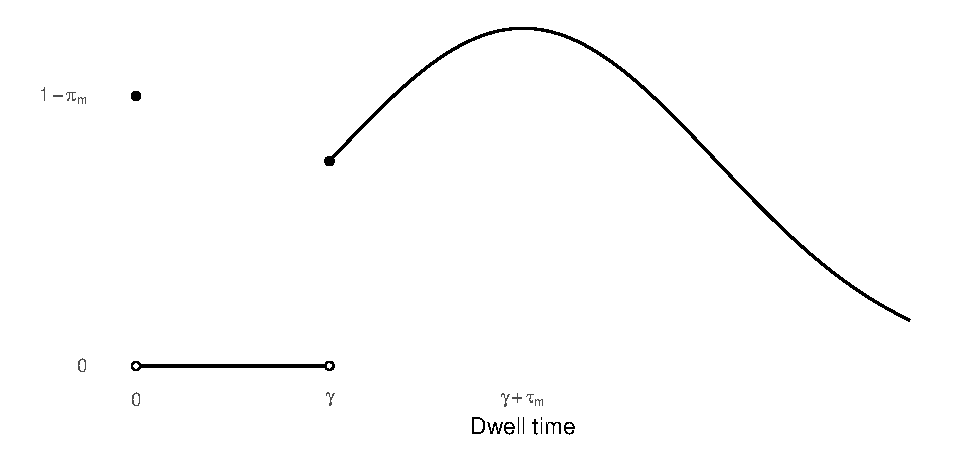
\includegraphics[width=.8\textwidth]{figure/eta_dwell_times-1} 

}

\caption[The \gls{pdf} of dwell time at a stop]{The \gls{pdf} of dwell time at bus stop $m$.}\label{fig:eta_dwell_times}
\end{figure}


\end{knitrout}


One other scenario for bus stops is a \emph{layover}, which is when a bus arrives early at a major stop\footnote{This is more common on longer routes in an attempt to keep them to schedule.} and waits until the scheduled departure time. In the \gls{gtfs} stop times table, layovers are denoted by an arrival time earlier than the corresponding departure time, as shown in \cref{tab:layover_times}. Again, under the particle filtering framework, this is simple enough to implement: if the particle arrives early, it waits until the scheduled departure time before leaving. However, it is not always the case that buses will wait for the layover, so we add a probability of adherence, similar to the stopping probability in \cref{eq:stop_pstop}. However, since this has greater implication for arrival time prediction, we defer the details for \cref{cha:prediction}.

\begin{knitrout}\small
\definecolor{shadecolor}{rgb}{0.969, 0.969, 0.969}\color{fgcolor}\begin{table}

\caption[Arrival times for a trip with a layover]{\label{tab:layover_times}Arrival times for a trip with a layover stop (marked with an asterix, $\star$). This is indicated in the \gls{gtfs} data by a departure time later than the arrival (in this case the difference is one second).}
\centering
\fontsize{8}{10}\selectfont
\begin{tabular}[t]{rll}
\toprule
Stop & Arrives & Departs\\
\midrule
1 & 19:30:00 & 19:30:00\\
2 & 19:30:36 & 19:30:36\\
3 & 19:31:33 & 19:31:33\\
4 & 19:32:04 & 19:32:04\\
5 & 19:32:59 & 19:33:00 *\\
6 & 19:33:42 & 19:33:42\\
7 & 19:34:14 & 19:34:14\\
\bottomrule
\end{tabular}
\end{table}


\end{knitrout}




\paragraph{Intersections}

Modelling intersections is much the same as bus stops, with a few differences:
\begin{enumerate}[i.]
\item the bus doors do not open, passengers do not get on or off, so there is no longer a $\gamma$ parameter;
\item the bus does not necessarily stop at the node location, since there may be a queue;
\item depending on the length of the queue and the type of intersection, the bus may require more than one ``light phase'' to pass through the intersection (for traffic lights), OR the bus may creep forward slowly (at uncontrolled (give-way) intersections and roundabouts).
\end{enumerate}
However, we had no reliable intersection location information available, so were unable to explore this component of the model thoroughly. Instead, I describe here a single behaviour but note that it could easily be modified in the future.

We model the wait time $w$ at intersection $\ell$ with an exponential distribution with rate $\intwait_\ell^{-1}$:
\begin{equation}
\label{eq:int_wait}
\pcwait_\ell \sim \Exp{\intwait_\ell^{-1}}.
\end{equation}
As at bus stops, the stopping outcome $\Iint_\ell$ is a Bernoulli trial with probability $\rho_\ell$,
\begin{equation}
\label{eq:int_stop_bern}
\Iint_\ell \sim \Bern{\rho_\ell},
\end{equation}
leading to an overall wait time of
\begin{equation}
\label{eq:int_total_wait}
\pwait_\ell = \Iint_\ell \pcwait_\ell.
\end{equation}
However, from point iii above, once the wait time is over, we conditionally allow the bus to move forward with the possibility of stopping again. In practice, this would be proportional to the distance of the vehicle from the intersection and other factors. As mentioned in \cref{sec:vp_data}, this is not as easy as it seems since observations may be linked to a waypoint at the intersection\footnote{Actually, in the middle of it.} instead of where the bus is, so we cannot determine the bus's distance from the intersection reliably.

\subsection{Likelihood}
\label{sec:pf-likelihood}

The second component of \gls{rbe} is the update step, which involves accounting for the likelihood of the data given the predicted state, $p(\Vobs_k | \Vstate_k)$. In the \pf{}, as discussed in \cref{sec:pf}, updating is performed by reweighting each of the particles based on their likelihoods, $p(\Vobs_k | \Vstate\vi_k)$, and then, if necessary, performing weighted resampling with replacement (importance resampling). That is,
\begin{equation}
\label{eq:vehicle_pf_update}
p(\Vstate_k | \Vobs_{1:k}) \approx
\sum_{i=1}^\Np
    \Pwt_{k}
    \DiracMeasure{\Vstate\vi_k}{\Vstate_k}
\end{equation}
where
\begin{equation}
\label{eq:vehicle_pf_reweight}
\Pwt_k = \frac{
    \Pwt_{k-1} p(\Vobs_k | \Vstate\vi_k)
}{
    \sum_{j=1}^\Np \Pwt[j]_{k-1} p(\Vobs_k | \Vstate\vi[j]_k)
}
\end{equation}


The likelihood function is where the \pf{} is superior in this application. Were we to model the vehicle's state with a \kf{}, we would need to somehow compare a distribution in one dimension (distance travelled) with an observation in two dimensions (\gls{gps} coordinate). \cite{Cathey_2003} used an optimisation technique to obtain an estimated observation of distance travelled based on the observation location, which they then used as data for their \kf{} implementation. However, as demonstrated in \cref{fig:lhood_obs}, there are situations where the ``maximised'' location may be wrong, in which case the resulting state will be eroneous.


The \pf{} effectively checks to see how plausible the observation is assuming each particle is the truth, allowing us to weight each particle by its plausibility. Since there are two types of data, two likelihood functions are required: one for \GPS{} observations, and a second for trip updates. There is no need to match the observations to distance: instead, each particle's state can be transformed into a \gls{gps} coordinate, making it directly compariable to the vehicle's reported location.


\subsubsection{GPS vehicle locations}
\label{sec:lhood_gps}

\begin{knitrout}\small
\definecolor{shadecolor}{rgb}{0.969, 0.969, 0.969}\color{fgcolor}\begin{figure}
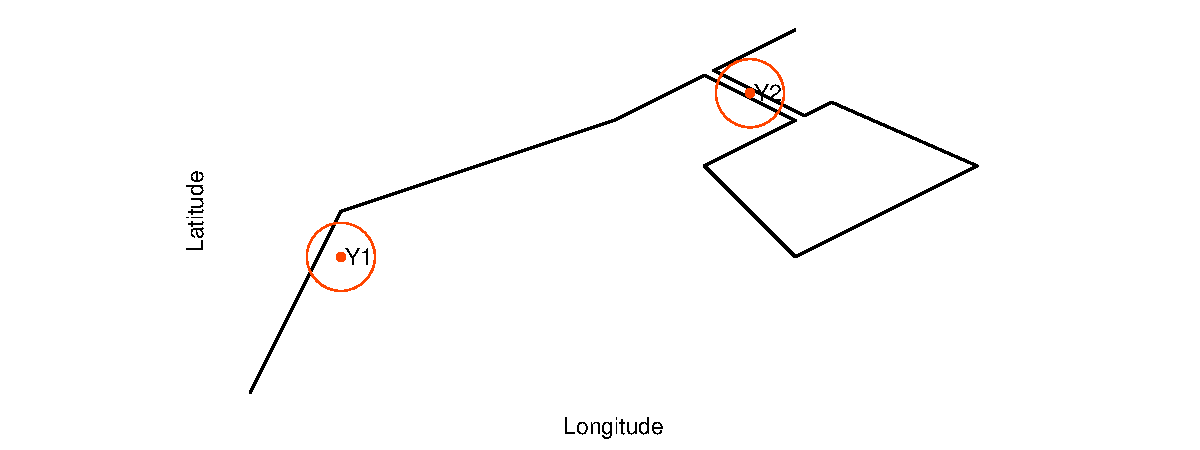
\includegraphics[width=\maxwidth]{figure/lhood_obs-1} \caption[Observations of vehicle on a simple path]{Observations of vehicle on a simple path. The red points indicate the reported GPS positions, with circles indicating the GPS error associated with each observation. Observation Y1 is easy to map to the route, while Y2 is more complicated and has two plausible, distinct locations.}\label{fig:lhood_obs}
\end{figure}


\end{knitrout}





For the \gls{gps} location update, the inherent \gls{gps} error, $\GPSerr$, needs to be filtered out to get better estimates of vehicle state. Examples of positions are shown in \cref{fig:lhood_obs}. A particle's likelihood should represent the geographical \emph{closeness} of the estimated position to the vehicle's reported position. We therefore want the likelihood to depend on the \emph{distance between the observed and predicted} vehicle locations. The first step to computing the likelihood is therefore
to calculate the GPS position of the \emph{particle}, $\Ppos\vi_k$, by using the \emph{measurement function},
\begin{equation}
\label{eq:pf_measurement_fun}
\Ppos\vi_k = \Vmeas(\Vstate\vi_k, \ShapePath)
\end{equation}
which is simply a deterministic function given the route's path, $\ShapePath$, which is a sequence of latitude-longitude pairs and the cumulative distance along the line. Once the geographical position of the particle is obtained, it is compared to the observed vehicle location, as shown in \cref{fig:gps_dist}.

\begin{knitrout}\small
\definecolor{shadecolor}{rgb}{0.969, 0.969, 0.969}\color{fgcolor}\begin{figure}

{\centering 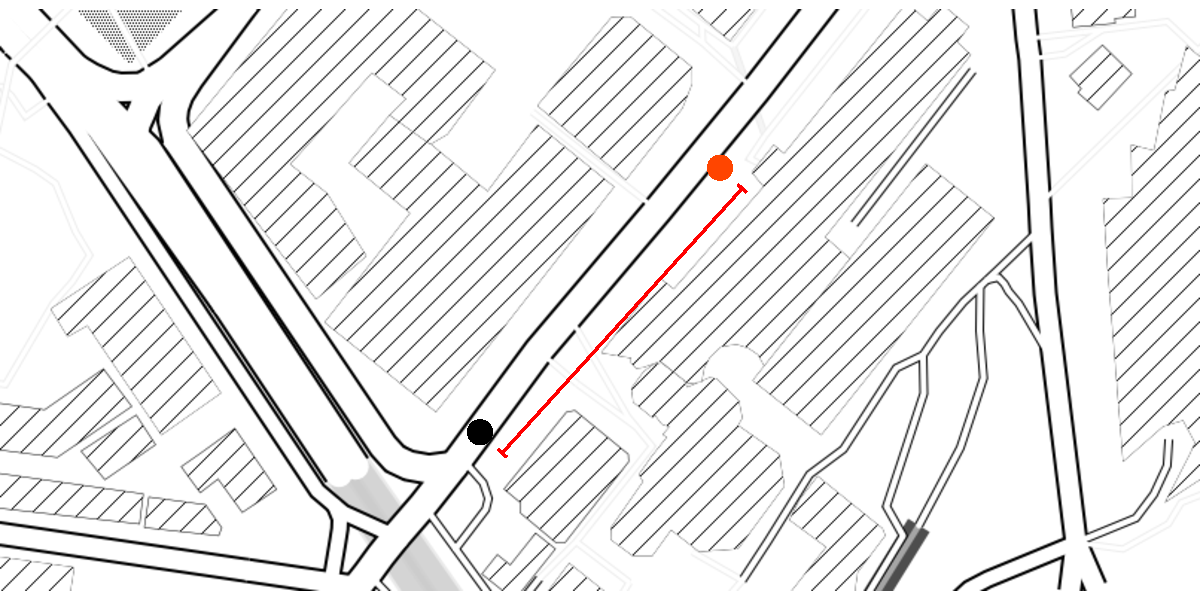
\includegraphics[width=0.8\textwidth]{figure/gps_dist-1} 

}

\caption[GPS distance between two points]{GPS distance between two points. The vehicle's reported location is shown in orange; one particle estimate of it's location is in black. The desired distance is denoted by the red line.}\label{fig:gps_dist}
\end{figure}


\end{knitrout}

Computing the distance between two GPS coordinates can achieved using several formulae, each with varying levels of accuracy. Since all of the distances are going to be (very) small, the \emph{Equirectangular projection} is sufficiently accurate for computing geographical distances \citep{cn}. This projection transforms the point $\Vobs_1 = \tvec{\Vlon_1, \Vlat_1}$, where latitude $\Vlat$ and longitude $\Vlon$ are in radians (the width of one longitudinal radian depends on latitude) onto a surface with meters on both axes, centered on the point $\Vobs_0 = \tvec{\Vlon_0, \Vlat_0}$ and using the Earth's radius $R = 6.371 \times 10^6$m,
\begin{equation}
\label{eq:equirectangular_projection}
\Vproj{\Vobs_1}{\Vobs_0} =
\begin{bmatrix} x \\ y \end{bmatrix} =
R \begin{bmatrix}
(\Vlon_1 - \Vlon_0) \cos \Vlat_0 \\
(\Vlat_1 - \Vlat_0)
\end{bmatrix}
\end{equation}
so that the distance between the points can easily be computed
using their \emph{euclidean distance}
\begin{equation}
\label{eq:obs_dist}
\dist{\Vobs_0, \Vobs_1} = \sqrt{x^2 + y^2}.
\end{equation}
This is shown visually in \cref{fig:gps_projection}.
Note that conversion from degrees to radians is achieved by
multiplying degrees by $\frac{\pi}{180}$.

\begin{knitrout}\small
\definecolor{shadecolor}{rgb}{0.969, 0.969, 0.969}\color{fgcolor}\begin{figure}

{\centering \subfloat[GPS coordinates\label{fig:gps_projection1}]{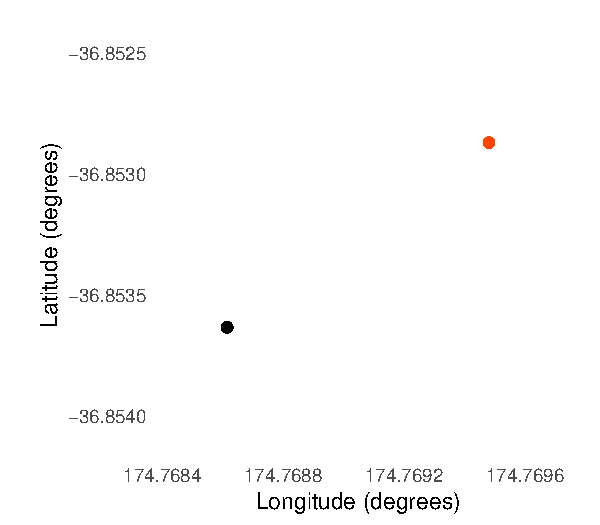
\includegraphics[width=0.49\textwidth]{figure/gps_projection-1} }
\subfloat[Projected points\label{fig:gps_projection2}]{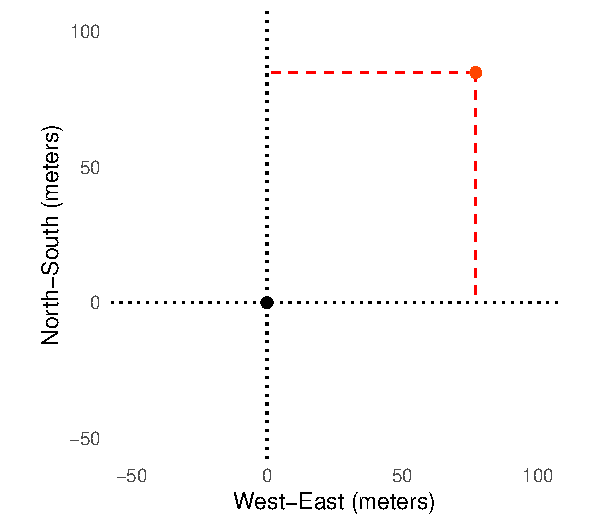
\includegraphics[width=0.49\textwidth]{figure/gps_projection-2} }

}

\caption[Equirectangular projection of GPS coordinates onto flat surface, allowing the distance from each particle to the observed location to easily be calculated]{Equirectangular projection of GPS coordinates onto flat surface, allowing the distance from each particle to the observed location to easily be calculated.}\label{fig:gps_projection}
\end{figure}


\end{knitrout}


Now that spherical observations can be compared on a flat surface,
it is necessary to assume that \GPS{} observations are distributed
as a multivariate random variable around the true position of the vehicle
on the ground,
with a \GPS{} error of $\GPSerr$,
and that the variation does not depend on direction.
That is, if the observation $\Vobs_k$ is projected using
\cref{eq:equirectangular_projection} conditional on the true position
$\Vmeas(\Vstate_k)$,
then the projected point will be a multivariate random variable
$\vec{r}_k \sim \Normal{\vec{0}}{\GPSerr \mat{I}}$.
The above, shown in \cref{fig:gps_error2},
can more simply be expressed by
\begin{equation}
% \label{eq:obs_projection}
\label{eq:gps_error_model}
\Vproj{\Vobs_k}{\Vmeas(\Vstate_k)} =
    \Vproj{\Vmeas(\Vstate_k)}{\Vmeas(\Vstate_k)} + \vec{r}_k
    = \vec{r}_k
\end{equation}

% \begin{equation}
% \Vobs_k = \Viproj{\vec{r}\vi_k}{\Vmeas(\Vstate\vi_k)}.
% \end{equation}

\begin{knitrout}\small
\definecolor{shadecolor}{rgb}{0.969, 0.969, 0.969}\color{fgcolor}\begin{figure}

{\centering \subfloat[GPS map error\label{fig:gps_error1}]{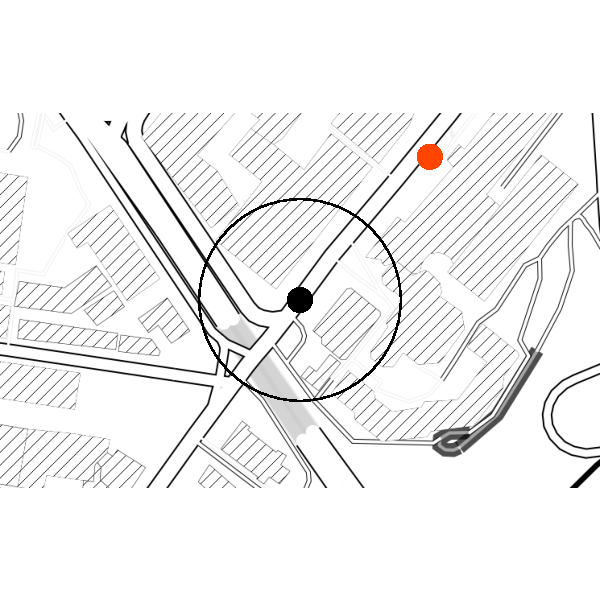
\includegraphics[width=0.49\textwidth]{figure/gps_error-1} }
\subfloat[Projected error\label{fig:gps_error2}]{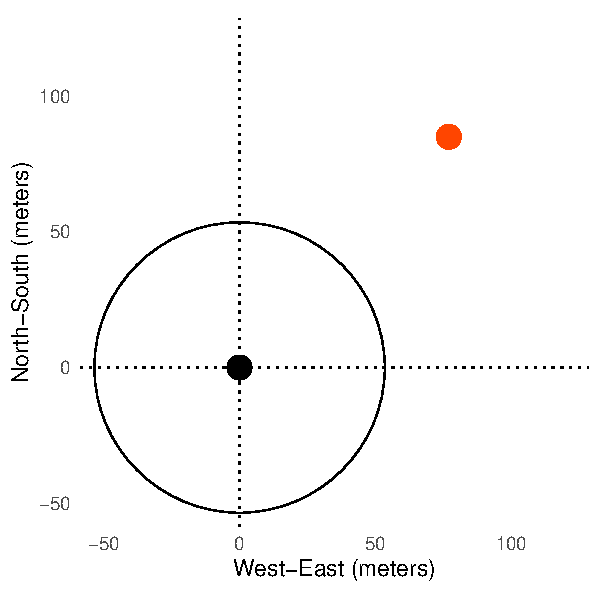
\includegraphics[width=0.49\textwidth]{figure/gps_error-2} }

}

\caption[GPS error is assumed to be circular on a map]{GPS error is assumed to be circular on a map.}\label{fig:gps_error}
\end{figure}


\end{knitrout}


From \cref{eq:equirectangular_projection,eq:obs_dist,eq:gps_error_model}
the distance between the true and observed locations
is the magnitude of the error $\vec{r}_k$,
\begin{equation}
\dist{\Vobs_k, \Vmeas(\Vstate_k)} = ||\vec{r}_k|| =
    \sqrt{r_{k1}^2 + r_{k2}^2}
\end{equation}
However, this error can also be expressed in terms of two independent,
standard normal random variables $z_1, z_2 \sim \Normal{0}{1}$,
such that $r_{jk} = \GPSerrSD z_j$ for $j = 1, 2$,
resulting in
\begin{equation}
\dist{\Vobs_k, \Vmeas(\Vstate\vi_k)} =
    \sqrt{(\GPSerrSD z_1)^2 + (\GPSerrSD z_2)^2} =
    \GPSerrSD \sqrt{z_1^2 + z_2^2}
\end{equation}
Since the distribution of two squared standard normal random variables is known
to be $\chi^2$ distributed with 2~degrees of freedom,
which is itself exponential with rate 0.5
\citep{cn},
then
\begin{equation}
\label{eq:sum_sq_dist}
z_1^2 + z_2^2 \sim \Exp{\frac{1}{2}}
\end{equation}
which, following the [fact] that if $X \sim \Exp{\theta}$,
then $cX \sim \Exp{\frac{\theta}{c}}$,
the squared distance between points is simply represented as
\begin{equation}
\label{eq:distance_distrib}
\dist{\Vobs_k, \Vmeas(\Vstate_k)}^2 \sim \Exp{\frac{1}{2\GPSerr}}
\end{equation}

So now, given a particle state estimate of $\Vstate\vi_k$,
the likelihood of a \GPS{} observation using only
the distance between two coordinates is given by
\begin{equation}
\label{eq:particle_lh_fun}
p(\Vobs_k | \Vstate\vi_k) =
    \frac{1}{2\GPSerr} \exp\left\{
        - \frac{\dist{\Vobs_k, \Vmeas(\Vstate\vi_k)}^2}{2\GPSerr}
    \right\}
\end{equation}
allowing the particles to be reweighted using \cref{eq:vehicle_pf_reweight}.
This is shown visually in \cref{fig:pf_wts}.


\begin{knitrout}\small
\definecolor{shadecolor}{rgb}{0.969, 0.969, 0.969}\color{fgcolor}\begin{figure}

{\centering 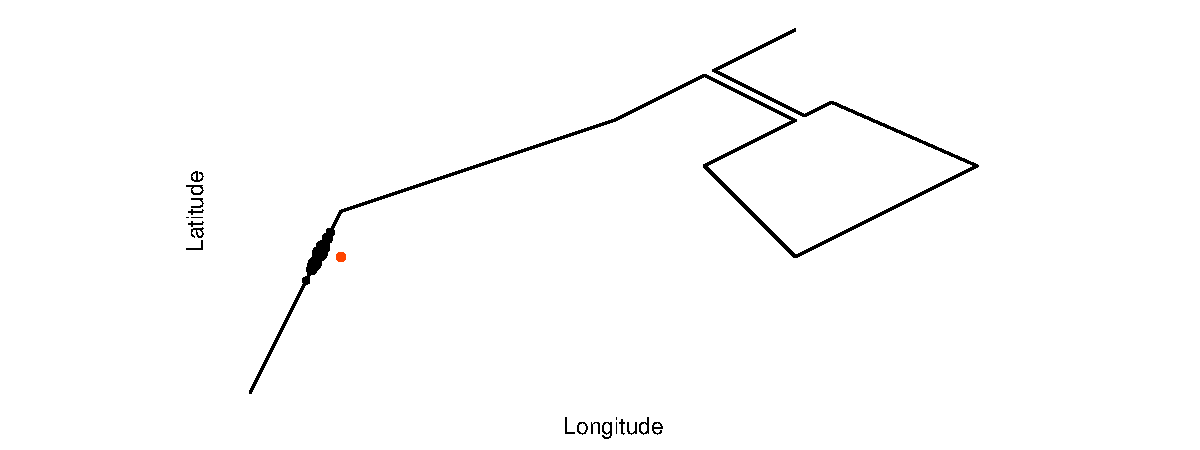
\includegraphics[width=\maxwidth]{figure/pf_wts-1} 

}

\caption[The \pf{} estimate of vehicle state after reweighting particles based on the likelihood, or distance from the observed location]{The \pf{} estimate of vehicle state after reweighting particles based on the likelihood, or distance from the observed location.}\label{fig:pf_wts}
\end{figure}


\end{knitrout}


\subsubsection{Trip updates}
\label{sec:lhood_trip}

As well as vehicle position updates from \GPS{} data, \GTFS{} provides trip updates from arrival and departure information. In many situations, it is difficult to infer a vehicle's trajectory based solely on \GPS{} data, and so trip updates are therefore an invaluable part of the update step. In this case, the \pf{} prediction step goes ahead as presented in \cref{sec:vehicle_model_trans}, but instead of then comparing the coordinates, the arrival or departure times are used to compute the liklelihood of the particles.


The trip update observations differ from the \GPS{} observations in that there are now three situations which can occur. The observation can be of an arrival time at stop $m$, $\Varr_m$, or it can be of a departure time, $\Vdep_m$. In the latter case, treatment of the observations depends on whether or not $\Varr_m$ was observed. This gives us three likelihood functions to derive,
\begin{itemize}
\item $p(\Varr_m | \Vstate_k)$, the arrival time likelihood function,
\item $p(\Vdep_m | \Vstate_k, \text{arrival missing})$, the departure time likelihood conditional
    on not having observed arrival time, and
\item $p(\Vdep_m | \Vstate_k, \text{arrival observed})$, the departure time likleihood conditional
    on having observed arrival time.
\end{itemize}


To compute the likelihood for these, we refer back to the dwell time model described in \cref{eq:stop_dwell_model,eq:stop_dwell_time}. Two additional parameters are also needed: the actual arrival time of the bus at stop $m$, $\Tarr_{m}$, and the measurement error of arrival time in seconds, $\TUerr$. The arrival time can be computed for each stop $m$ directly from the model (i.e., via interpolation). The departure time is then computed by summing the arrival and dwell times.


The observed arrival and departured times, denoted $\Varr_m$ and $\Vdep_m$, respectively, are assumed to each be normally distributed, with mean and variance determined by the described model. For arrival time, this is simply
\begin{equation}
\label{eq:tu_arr_lhood}
\Varr_m \sim \Normal{\Tarr_{mr}}{\TUerr}.
\end{equation}
and for departure time,
\begin{equation}
\label{eq:tu_dep_lhood}
\Vdep_m \sim \Normal{\Tarr_m + \pdwell_m}{\TUerr}
\end{equation}


In our \pf{} implementation, each observation will be processed individually; in situations where more than one type of observation is recieved, they are processed in chronological order and the particles reweighted between each. The necessary likelihood component for \cref{eq:vehicle_pf_reweight} is therefore
\begin{equation}
\label{eq:tu_obs_lhood}
p(\Vobs_k | \Vstate\vi_k) =
\begin{cases}
\frac{1}{\sqrt{2\pi\TUerr}}
    \exp\left\{
        -\frac{(\Varr_m - \Tarr_m)^2}{2\TUerr}
    \right\} & \text{for arrival times} \\
\frac{1}{\sqrt{2\pi\TUerr}}
    \exp\left\{
        -\frac{(\Vdep_m - \Tarr\vi_m - \pdwell\vi_m)^2}{2\TUerr}
    \right\} & \text{for departure times}
\end{cases}
\end{equation}
which allows the particle sample to be reweighted according to the temporal difference in arrival and departure times. This is demonstrated in \cref{fig:tu_update}.

\begin{knitrout}\small
\definecolor{shadecolor}{rgb}{0.969, 0.969, 0.969}\color{fgcolor}\begin{figure}

{\centering 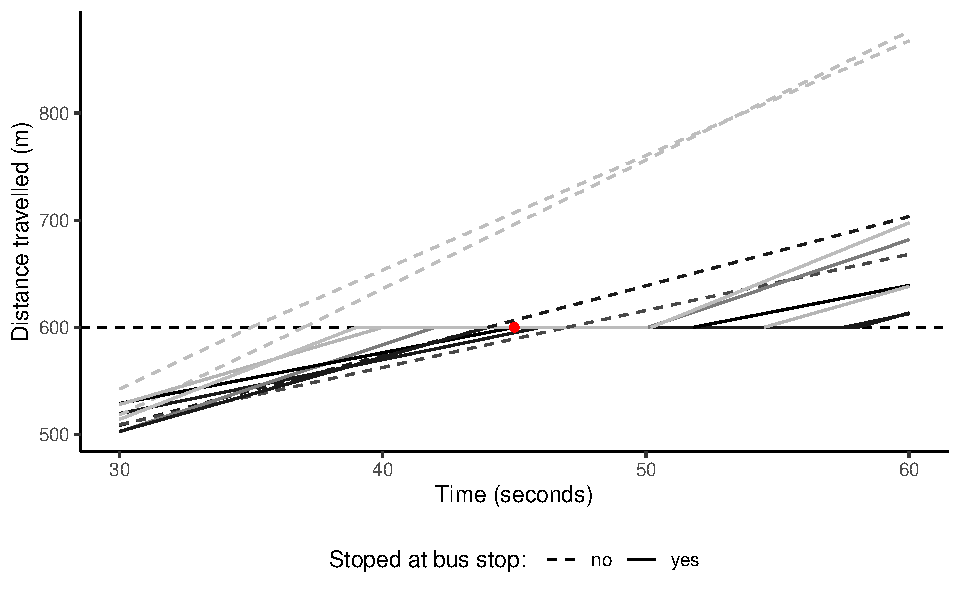
\includegraphics[width=0.8\textwidth]{figure/tu_update-1} 

}

\caption[Particle's travelling past an intermediate stop with an arrival time observation (red point)]{Particle's travelling past an intermediate stop with an arrival time observation (red point). Solid lines represent particles that stopped, while dashed lines indicate the particle drove straight past the stop. The lines are coloured by their resepective weights according to the likelihood based on the observed arrival time (red dot), where greyer lines have less weight.}\label{fig:tu_update}
\end{figure}


\end{knitrout}


\section{Estimating road speeds}
\label{sec:vehicle_speeds}

Now that we have estimated the necessary vehicle states and their respective trajectories, we can infer each vehicle's \emph{average speed} along road segment $\ell$ of its current route, $\Vtt_{\ell}$. These estimates are later used to update the \emph{road network state} (\cref{cha:network_model}) and ultimately estimate arrival times (\cref{cha:prediction}).


Estimation of average road speed is performed by first computing the \emph{travel time} along each road segment as the bus traverses the network. To do so, we record the time when the vehicle starts and ends each segment, $\Vsegstart_\ell$ and $\Vsegend_\ell$, respectively, and take the difference to obtain the travel time in seconds. By using a particle filter, we record these values for each particle as it is transitioned to each new state. Finally, transforming to average speed uses the length of the segment, $\Tseglen_\ell$, in meters, and the standard speed formula ($\text{speed} = \frac{\text{distance}}{\text{time}}$):
\begin{equation}
\label{eq:vehicle_avg_speed}
\Vtt\vi_\ell = \frac{\Tseglen_\ell}{{\Vsegend}\vi_\ell - {\Vsegstart}\vi_\ell}.
\end{equation}


Since estimating \cref{eq:vehicle_avg_speed} is straightforward for each particle, the posterior distribution of the vehicle's average travel time along segment $\ell$, given all observations up to and including time $\Vtime_k$, is approximated using the Dirac delta measure,
\begin{equation}
\label{eq:pf_speed_dist}
p(\Vtt_\ell \cond{} \Vobs_{1:k}) \approx
\sum_{i=1}^\Np \Pwt_k \DiracMeasure{\Vtt\vi_\ell}{\Vtt_\ell}.
\end{equation}
In situations where only some particles have completed travel along a segment, the application waits until the next iteration to re-check that all particles have completed it and, if so, the average speed is calculated.


\subsection{Simulation study}
\label{eq:pf_simulation_study}

To assess the accuracy of the models presented in \cref{sec:vehicle_model}, vehicle simulations were performed with known road speeds while tracking the vehicle along the route. Three different sampling methods were used to obtain observations:
\begin{itemize}
\item uniform sampling with 10~second intervals;
\item uniform sampling with 30~second intervals; and
\item non-uniform sampling at nodes.
\end{itemize}
As mentioned in \cref{sec:vp_data}, the last of these is, in fact, a common feature of the Auckland Transport data; we discuss the complications further in \cref{sec:pf_implementation}. In each simulation, we implemented the three variations of the transition function: $\Vtrans_{A1}$, $\Vtrans_{A2}$, and $\Vtrans_{A3}$.


The posterior mean travel time was used to examine and compare the estimation accuracy of the models, which is simple to calculate from the particle filter estimates of travel time using the weighted mean of the sample (\cref{app:particle-summaries}):
\begin{equation}
\label{eq:pf_travel_time_mean}
\bar\Vtt_\ell =
\E{\Vtt_\ell | \Vobs_{1:k}} =
\sum_{i=1}^\Np \Pwt_k \Vtt\vi_\ell.
\end{equation}


To evaluate and compare the estimation performance of the models, we use \gls{rmse} and \gls{mae} (defined in \cref{app:error-functions}).


\subsubsection{Simulation A: general vehicle model}
\label{sec:vehicle_sim_A}





The simulated data, shown in \cref{fig:sim1_graph}, uses the transition model described by $\Vtrans_{A3}$ to simulate a vehicle trajectory ignoring bus stops. Observations are obtained using three sampling methods: uniform sampling with high and low frequency, and non-uniform sampling, which is more in line with how the Auckland Transport data is collected.


The goal of the simulation is to estimate the vehicle's average speed along several road segments, as well as the associated uncertainty. The simulation was performed in \Rstats{} \citep{rcore} using $\Np = 2000$ particles per vehicle, and so the implementation is slightly different from the \Cpp{} one defined in \cref{sec:pf_implementation}.

\begin{knitrout}\small
\definecolor{shadecolor}{rgb}{0.969, 0.969, 0.969}\color{fgcolor}\begin{figure}
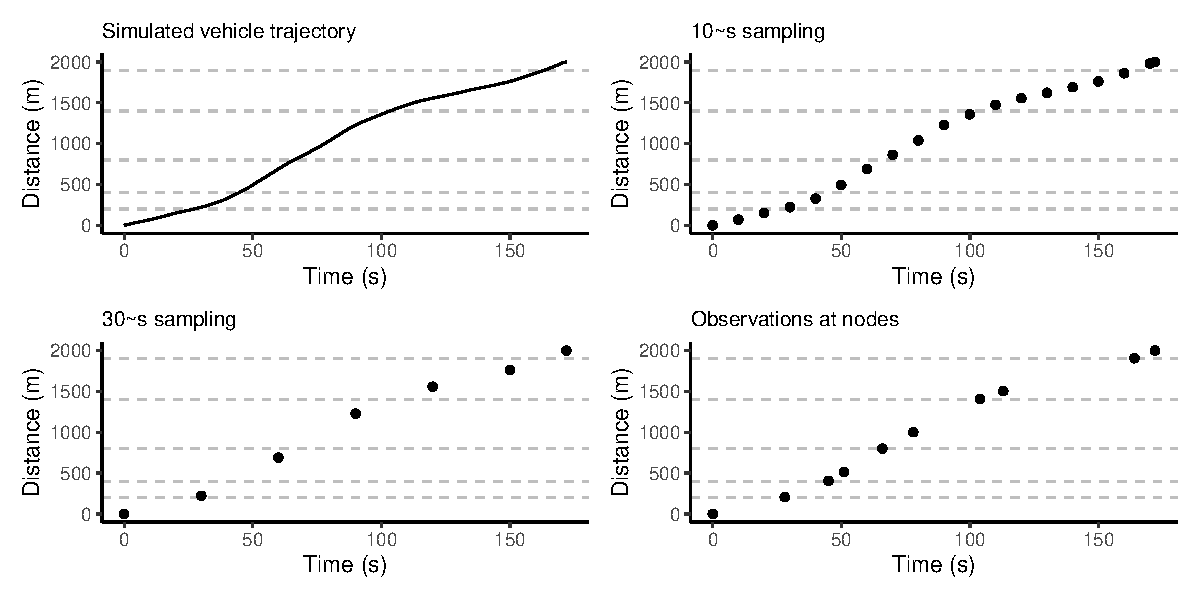
\includegraphics[width=\linewidth]{figure/sim1_graph-1} \caption[Vehicle trajectory with sampled observations for simulation A]{A simulated vehicle trajectory (top left) for simulation A along five road segments (dashed grey lines). Observations are sampled using three techniques (see text).}\label{fig:sim1_graph}
\end{figure}


\end{knitrout}

\begin{knitrout}\small
\definecolor{shadecolor}{rgb}{0.969, 0.969, 0.969}\color{fgcolor}\begin{figure}
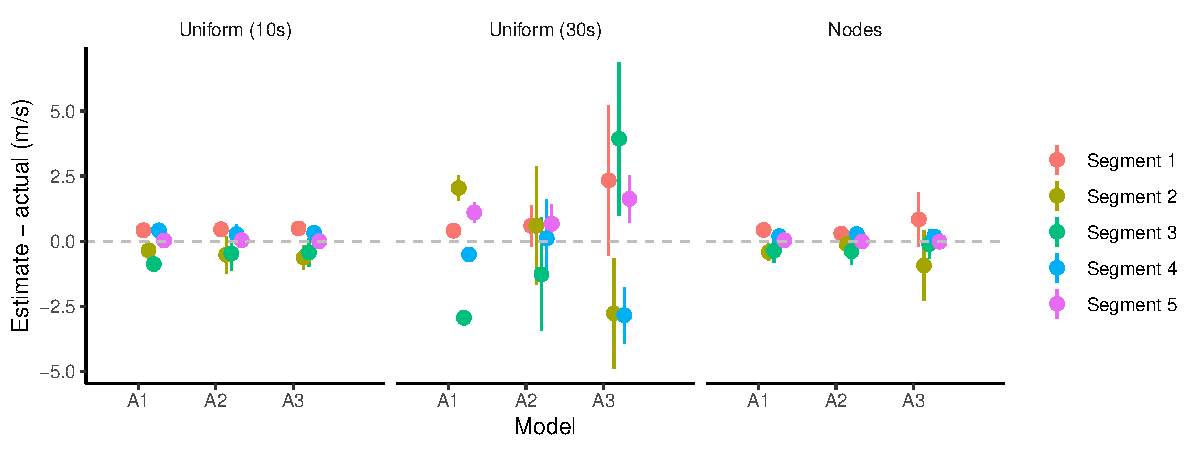
\includegraphics[width=\linewidth]{figure/sim1_pf-1} \caption[Results for simulation A]{Simulation A results for the three models (A1, A2, A3) applied to the data from three sampling methods using $\Np=2000$ particles. Shown is the travel time prediction error along with its standard deviation.}\label{fig:sim1_pf}
\end{figure}


\end{knitrout}


The results of the simulation applied to the data displayed in \cref{fig:sim1_graph} is shown in \cref{fig:sim1_pf}. Under the high-frequency uniform sampling method, all models perform similarly with high precision (the errors are all close to zero) and accuracy (the uncertainty is small enough that the error bars are barely visible). For the low-frequency sampling, however, model A2 shows slightly better precision than A1 and A3. Finally, for sampling at nodes, the models all perform similarly.



To further examine the comparative performance of the models, we repeated the simulation 100~times using the same segments and sampling points, but varying the underlying trajectory of the vehicle, with the results displayed in \cref{fig:sim1_pf_full}. Models A1 and A2 have better accuracy than A3. Most obviously, however, is that the sampling rate significantly affects accuracy. An overall comparison of \gls{rmse} and \gls{mae} are displayed in \cref{tab:sim1_pf_full}, which affirms the findings that A3 is less accurate than the other methods  (except under high-frequency sampling where they all perform similarly).


\begin{knitrout}\small
\definecolor{shadecolor}{rgb}{0.969, 0.969, 0.969}\color{fgcolor}\begin{figure}
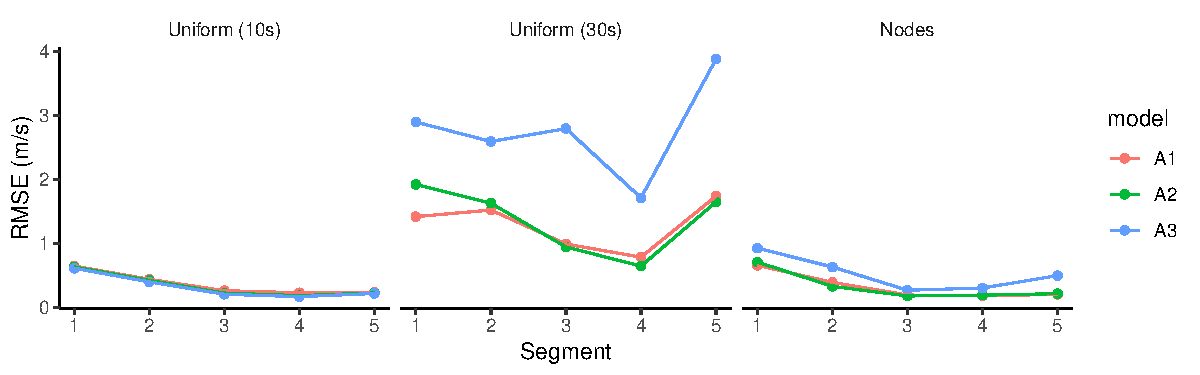
\includegraphics[width=\linewidth]{figure/sim1_pf_full-1} \caption[Results for simulation A replicated 100~times]{Speed estimation results for 100 simulations. In each the vehicle trajectory was simulated using a different seed and speed estimated by the mean of the particles, which is compared to the true speed using \gls{rmse}.}\label{fig:sim1_pf_full}
\end{figure}

\begin{table}

\caption{\label{tab:sim1_pf_full}RMSE and MAE of average speed estimation for simulation A for three models and three sampling techniques.}
\centering
\fontsize{8}{10}\selectfont
\begin{tabular}[t]{llrr}
\toprule
Sampling method & Model & RMSE (m/s) & MAE (m/s)\\
\midrule
Uniform (10s) & A1 & 0.40 & 0.27\\
 & A2 & 0.38 & 0.26\\
 & A3 & 0.36 & 0.24\\
\midrule
Uniform (30s) & A1 & 1.34 & 0.95\\
 & A2 & 1.44 & 1.01\\
 & A3 & 2.87 & 2.07\\
\midrule
Nodes & A1 & 0.38 & 0.25\\
 & A2 & 0.38 & 0.25\\
 & A3 & 0.58 & 0.36\\
\bottomrule
\end{tabular}
\end{table}


\end{knitrout}



\subsubsection{Simulation B: bus stop model}
\label{sec:vehicle_sim_B}

In the previous simulation, we assumed the vehicle travelled along the route without stopping. Now, we add bus stop behaviour to the model, as shown in \cref{fig:sim2_graph}. In the simulated data, the bus stops at all stops with unknown dwell time, and we use $\pi=0.5$ for the stopping probability in the particle filter when estimating vehicle state. The sampling is the same as before: 10~second and 30~second rates, as well as observations at nodes (intersections and bus stops). In this simulation, models B1, B2, and B3 are modified versions of A1, A2, and A3, respectively, but include bus stopping behaviour from \cref{sec:vehicle_model_nodes}.




\afterpage{\clearpage}

The results of the second simulation are shown in \cref{fig:sim2_pf}, where we see somewhat similar results as before: the models perform equally well under high-frequency uniform sampling, with lower precision and accuracy under low-frequency sampling. For sampling at nodes, the models perform similarly.

\begin{knitrout}\small
\definecolor{shadecolor}{rgb}{0.969, 0.969, 0.969}\color{fgcolor}\begin{figure}
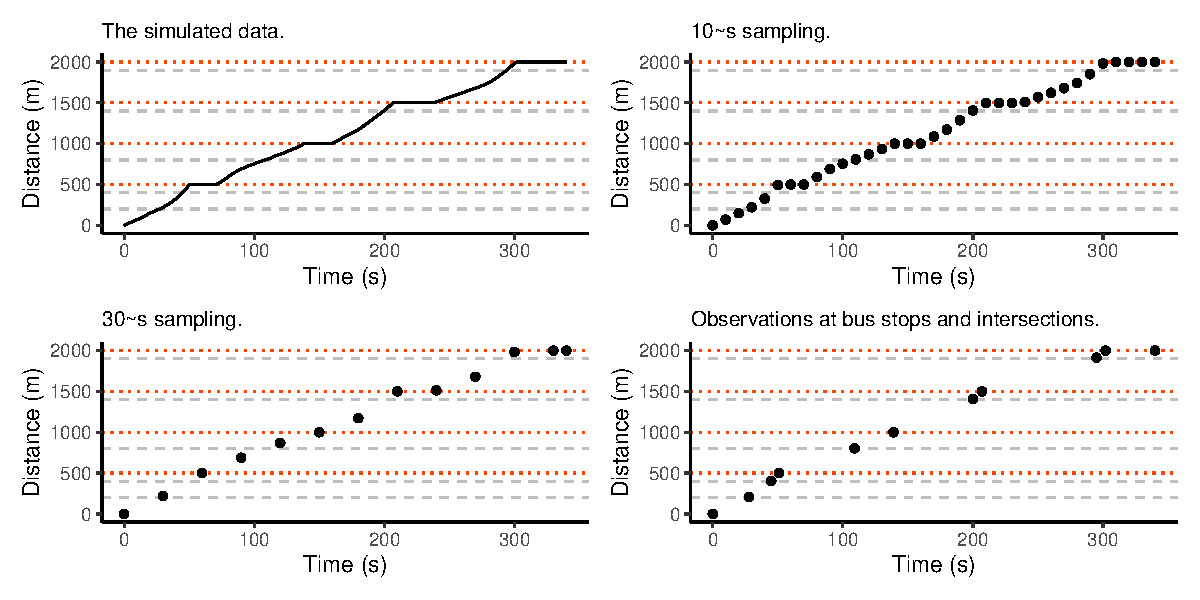
\includegraphics[width=\linewidth]{figure/sim2_graph-1} \caption[Vehicle trajectory with sampled observations for simulation B]{A simulated vehicle trajectory (top left) for simulation B along five road segments (dashed grey lines) with four stops (dotted orange lines). Observations are sampled using three techniques (see text).}\label{fig:sim2_graph}
\end{figure}


\end{knitrout}

\begin{knitrout}\small
\definecolor{shadecolor}{rgb}{0.969, 0.969, 0.969}\color{fgcolor}\begin{figure}[p]
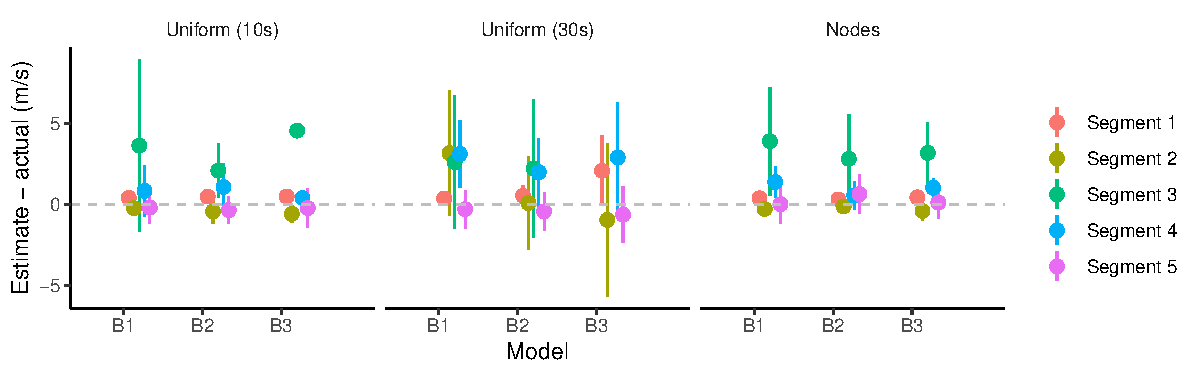
\includegraphics[width=\linewidth]{figure/sim2_pf-1} \caption[Results for simulation B]{Simulation B results for the three models (B1, B2, B3) applied to the data from three sampling methods using $\Np=2000$ particles. Shown is the travel time prediction error along with its standard deviation.}\label{fig:sim2_pf}
\end{figure}


\end{knitrout}





\begin{knitrout}\small
\definecolor{shadecolor}{rgb}{0.969, 0.969, 0.969}\color{fgcolor}\begin{figure}[p]
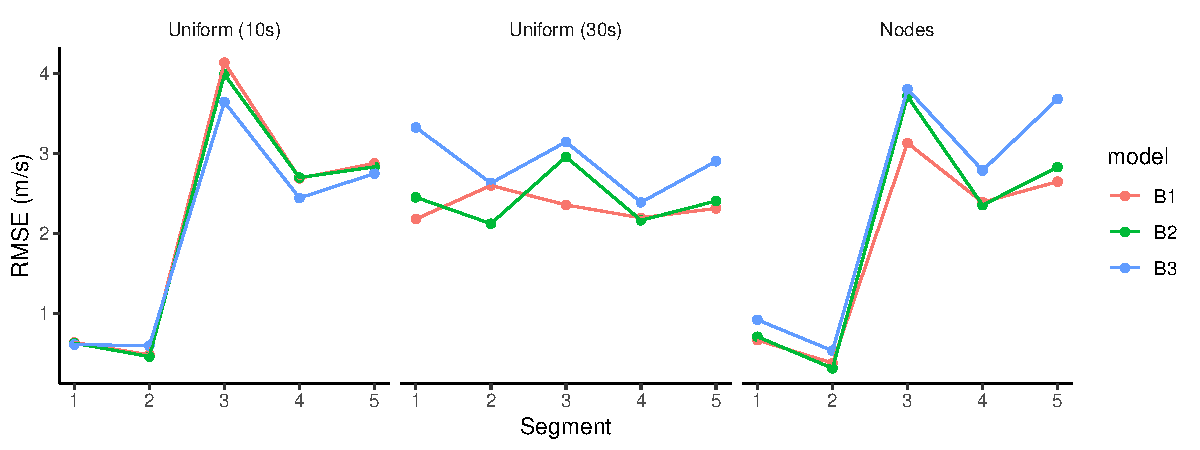
\includegraphics[width=\maxwidth]{figure/sim2_pf_full-1} \caption[Results for simulation B replicated 100~times]{Speed estimation results for 100 simulations. In each the vehicle trajectory was simulated using a different seed and speed estimated by the mean of the particles, which is compared to the true speed using \gls{rmse}.}\label{fig:sim2_pf_full}
\end{figure}

\begin{table}[p]

\caption{\label{tab:sim2_pf_full}RMSE and MAE of average speed estimation for simulation B for three models and three sampling techniques.}
\centering
\fontsize{8}{10}\selectfont
\begin{tabular}[t]{llrr}
\toprule
Sampling method & Model & RMSE (m/s) & MAE (m/s)\\
\midrule
Uniform (10s) & B1 & 2.56 & 1.40\\
 & B2 & 2.51 & 1.35\\
 & B3 & 2.34 & 1.35\\
\midrule
Uniform (30s) & B1 & 2.34 & 1.58\\
 & B2 & 2.43 & 1.63\\
 & B3 & 2.90 & 2.14\\
\midrule
Nodes & B1 & 2.15 & 1.31\\
 & B2 & 2.36 & 1.35\\
 & B3 & 2.70 & 1.57\\
\bottomrule
\end{tabular}
\end{table}


\end{knitrout}





Repeating the simulation 100~times with different vehicle trajectories, we can better compare the models (\cref{fig:sim2_pf_full}). Uncertainties are now much higher, on average, particularly under low-frequency sampling. The models all perform similarly, though B3 has the worst accuracy overall. \Cref{tab:sim2_pf_full} compares the estimates numerically using \gls{rmse} and \gls{mae}, where we see that within each sampling method the errors are similar. Models B1 and B2 perform similarly, while B3 is again consistently worse except under high-frequency sampling.




\phantom{\gls{rmse} \gls{mae}}


\section{Implementing the \rt{} \pf{}}
\label{sec:particle-filter}


The next major step in this work was to implement the model in real-time using C++. Our implementation involves a single call from the R package \verb+transitr+ which commences an infinite loop within C++ which
\begin{enumerate}
\item fetches the lastest observations,
\item attaches them to an existing vehicle, or creates a new one,
\item updates or initialises vehicle states using the particle filter model described in \cref{sec:vehicle_model}, and
\item estimates average road speeds as vehicles traverse the network as described in \cref{sec:vehicle_speeds},
\end{enumerate}
as displayed in \cref{fig:program_flow}. During the process of coding up our implementation (\cref{sec:pf_implementation}), we inevitably ran into issues, some of which are related to computational complexity, while others are due to imperfections with the data (see \cref{sec:pf_issues}). Once the implementation was complete, we needed to estimate the parameters (such as system noise and measurement error) for the model.


In order to assess the \rt{} performance of the model and our \pf{} implementation, we created a virtual \rt{} server which serves historical data. This means we can both process the data faster---we do not need to wait in \rt{} for new observations---and allows us to run the model with different settings and parameter values for comparison. We used (a subset of) data from Tuesday 8~October~2018 for the simulations used in \cref{sec:pf_issues,sec:pf_params}, which were carried out on a virtual machine with 8~Intel Xeon 3.00GHz CPU cores and 32~GB of memory, running Ubuntu 16.04 and R 3.4.1. The results themselves were processed locally using R 3.6.0. These results were published in \citet{Elliott_2020}.





\subsection{C++ particulars}
\label{sec:pf_implementation}

The general construction of the particle filter is straightforward and involves creating \class{Vehicle} and \class{Particle} objects (as well as the \gls{gtfs} objects described in \cref{sec:gtfs}). The \class{Vehicle} objects are stored within an \verb+std::unordered_map+ using their \gls{gtfs} \verb+vehicle_id+ as the key.

When a vehicle is first observed, a new \class{Vehicle} is created and inserted into the map. Then its state is initialised by creating a vector of $\Np$ \class{Particle} objects, each of which is assigned a speed between 0 and 30 m/s, and a distance based on the observation: for GPS observations, map matching is used to determine the approximate location, around which the particles are scattered. In situations where there are multiple candidate locations, particles are distributed uniformly between the minimum and maximum likely distances. For trip updates, the particles are placed at the appropriate stop. When new data for an existing vehicle is observed, the \class{Vehicle}'s relevant properties are updated (such as position and timestamp). Then each \class{Particle} is mutated using the transition function from \cref{sec:vehicle_model} and reweighted according to the likelihood function (\cref{sec:pf-likelihood}). If the effective sample size drops below the threshold $\Nthres=\frac{\Np}{4}$, the state is resampled with replacement and particle weights reset to $\frac{1}{\Np}$. See \cref{app:particle-resampling} for details on particle resampling.

Since the vehicles are modelled independently, and they only need to read from the \gls{gtfs} object (not modify it) the vehicle update step is easily parallelised to use $\tilde M$~cores using the \prog{OpenMP} library \citep{OMP}. This enables up to an $\tilde M$-fold increase in the speed of this step.

Once the update is complete, the segment index of all particles is obtained, and the \emph{minimum} is used as the vehicle's \emph{current segment}. If this is greater than it was at the end of the previous iteration, the average speed along all intermediate segments is computed by using \verb+std::accumulate+,
\begin{lstlisting}
double avg_speed = std::accumulate(state.begin (), state.end (), 0.0,
  [](double x, Particle& p) {
    return x + p.weight () * p.segment_speed.at (seg_index);
  });
\end{lstlisting}\pagebreak
along with the variance,
\begin{lstlisting}
double var_speed = std::accumulate(state.begin (), state.end (), 0.0,
  [&avg_speed](double x, Particle& p) {
    return x + p.weight () *
      pow (p.segment_speed.at (seg_index) - avg_speed, 2.0);
  });
\end{lstlisting}
These observations are then passed to the relevant \class{Segment} object which contains a vector of new data (used in chapter 4). The \class{Vehicle} object contains a pointer to its \class{Trip}, which has a list of \class{Segment} objects:\footnote{Note that we must still ensure each pointer exists before proceeding, as mentioned in \cref{sec:rt-implementation}.}
\begin{lstlisting}
trip ()->segments ().at (seg_index)->push_data (avg_speed, var_speed);
\end{lstlisting}

At this point, we have completed the modelling of the vehicle's state and obtained estimates of any available road speed information.

\subsection{Real-time performance of the \pf{}}
\label{sec:pf_issues}



The two components of the model to assess are the iteration timings and the performance of the particle filter itself. That is, does the program run fast enough to be feasible in real-time, and is the model (and its \pf{} implementation) capable of modelling transit vehicles in real-time?


\paragraph{Is the particle filter fast enough?}
At peak hour on a typical weekday morning, there can be in excess of 1000~buses operating in Auckland. This leads to having more than $1000\Np$~particles in memory, each being mutated and reweighted approximately once every 30~seconds or so. By varying $N$, we can control how quickly each set of observations is processed. \Cref{fig:pf_timings} shows the average timings of the vehicle model component of our application, as well as the average time per particle for varying $N$. More particles require more processing power, though there is additional overhead during the \emph{resampling} phase. Limiting the frequency of resampling is therefore necessary to make the program run faster, which is why we use the effective sample size, $\Neff$, described in \cref{sec:pf} on \cpageref{eq:Neff}.


\begin{knitrout}\small
\definecolor{shadecolor}{rgb}{0.969, 0.969, 0.969}\color{fgcolor}\begin{figure}

{\centering 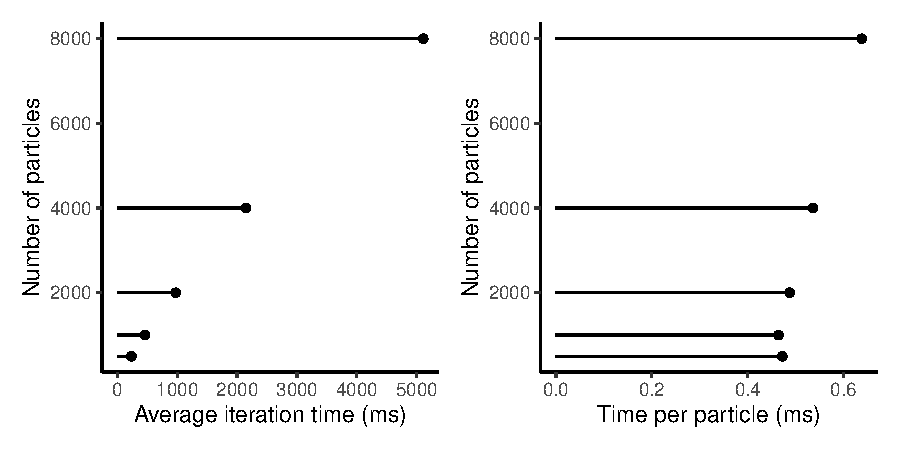
\includegraphics[width=.8\textwidth]{figure/pf_timings-1} 

}

\caption[Timings of the particle filter implemention for varying number of particles]{Timings of the particle filter implemention for varying number of particles. Left: the average iteration time (wall clock). Right: the average time per particle.}\label{fig:pf_timings}
\end{figure}


\end{knitrout}


\paragraph{How does the model perform?}





To assess how well our model performs in real-time, we repeated the simulation with a range of values of system noise $\Vnoise$, \gls{gps} error $\GPSerr$, and the number of particles $\Np$. For each simulation, we computed \emph{proportional effective sample size}, \emph{degeneration rate}, and \emph{relative variance}.

The \emph{proportional effective sample size} is the effective sample size relative to $N$, $\tilde N_\text{eff} = \frac{\Neff}{\Np}$. The higher this value, the less often the vehicle's state needs resampling, decreasing the average iteration time. \Cref{fig:model_performance_neff} shows the effect of $\Np$, system noise, and \gls{gps} error on $\tilde N_\text{eff}$. The most striking relationship is between $\tilde N_\text{eff}$ and \gls{gps} error: for larger error, more particles retain a high likelihood, and so the total weight is more evenly distributed. Conversely, larger values of system noise result in more variation between particles, leading to fewer particles ending near the observation position and decreasing $\tilde N_\text{eff}$.

\begin{knitrout}\small
\definecolor{shadecolor}{rgb}{0.969, 0.969, 0.969}\color{fgcolor}\begin{figure}

{\centering 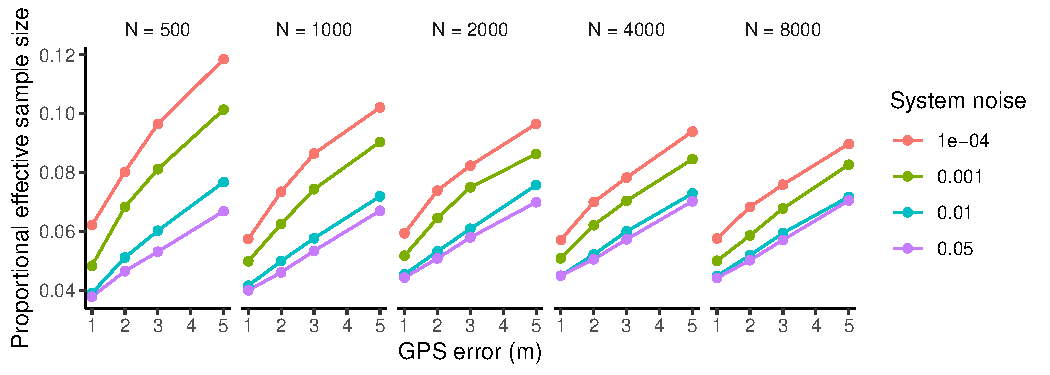
\includegraphics[width=\textwidth]{figure/model_performance_neff-1} 

}

\caption[Proportional effective sample size for varying values of GPS error, system noise, and number of particles]{Proportional effective sample size for varying values of GPS error, system noise, and number of particles.}\label{fig:model_performance_neff}
\end{figure}


\end{knitrout}


The \emph{degeneration rate} is the proportion of samples in which no particles end near the vehicle's reported position. In this case, all the particle likelihoods tend to zero, so the weights become undefined, resulting in the need to reinitialise the vehicle's state which results in the loss of any vehicle speed information along the most recently travelled road segment(s). We see from \cref{fig:model_performance_degen} that increasing \gls{gps} error or the number of particles reduces degeneration rate while increasing system noise shows a negligible reduction in degeneration rate. Larger \gls{gps} error means that particles do not need to end as close to the observed location to have a positive likelihood while increasing $\Np$ means more chance for a particle to end near the true bus.

\begin{knitrout}\small
\definecolor{shadecolor}{rgb}{0.969, 0.969, 0.969}\color{fgcolor}\begin{figure}

{\centering 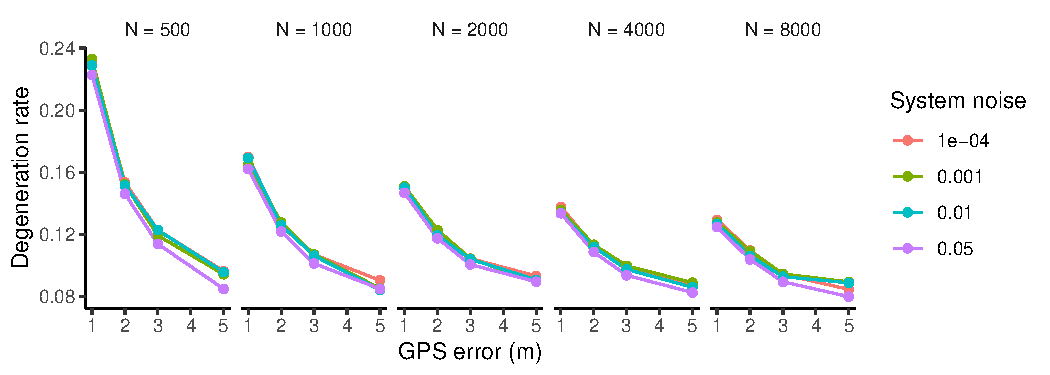
\includegraphics[width=\textwidth]{figure/model_performance_degen-1} 

}

\caption[Degeneration rate for varying values of GPS error, system noise, and number of particles]{Degeneration rate for varying values of GPS error, system noise, and number of particles.}\label{fig:model_performance_degen}
\end{figure}


\end{knitrout}

Finally, we have \emph{relative speed variance} along roads, which we use to compare the precision of the various models. It is the ratio of variance for a single simulation compared to the overall variance for all simulations. Let $\vec z_\ell^{e,s}$ be a vector of all vehicle speeds along road segment $\ell$ during the simulation with \gls{gps} error and system noise equal to $e$ and $s$, respectively. The ratio of the variance of speed for the single simulation compared to all simulations along one single road segment is given by
\begin{equation}
\label{eq:rel_speed_var_ratio}
v_\ell^{e,s} =
\frac{
    \mathrm{Var}(\vec z_\ell^{e,s})
}{
    \mathrm{Var}(\cup_e\cup_s \vec z_\ell^{e,s})
}.
\end{equation}
That is, for each segment in each simulation, we have a value representing whether this simulation estimates speed more or less accurately. We then compute the average ratio for all $L$ road segments,
\begin{equation}
\label{eq:rel_speed_var}
\bar v^{e,s} = \frac{1}{L} \sum_{\ell=1}^L v_\ell^{e,s}.
\end{equation}
A small value of $\bar v^{e,s}$ tells us that, on average, the simulation with \gls{gps} error $e$ and system noise $s$ estimates road speed \emph{with greater precision} than the other simulations. \Cref{fig:model_performance_var} presents these results, where we see the greatest effect on relative variance caused by increasing \gls{gps} error. Increasing $\Np$ produces a small decrease, and changes to system noise show no discernible effect.


\begin{knitrout}\small
\definecolor{shadecolor}{rgb}{0.969, 0.969, 0.969}\color{fgcolor}\begin{figure}

{\centering 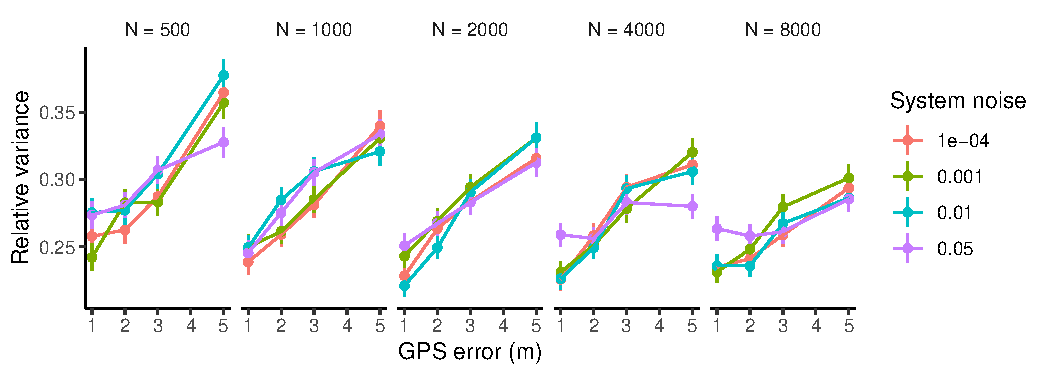
\includegraphics[width=\textwidth]{figure/model_performance_var-1} 

}

\caption[Relative speed variance for varying values of GPS error, system noise, and number of particles]{Relative speed variance for varying values of GPS error, system noise, and number of particles.}\label{fig:model_performance_var}
\end{figure}


\end{knitrout}


The results displayed in \cref{fig:model_performance_neff,fig:model_performance_degen,fig:model_performance_var} present a \emph{trade-off} between performance and estimation. Increasing \gls{gps} error increases the effective sample size, which reduces the frequency of resampling and speeds up each iteration. We also see a reduction in the rate of degeneration, which implies the particle filter is less likely to lose the vehicle and provide the desired speed estimates. However, increasing \gls{gps} error also increases the relative uncertainty of speed estimates. Increasing the number of particles generally results in a reduction in both degeneration rate and relative uncertainty, but, from \cref{fig:pf_timings}, this comes at the cost of increased computational demand.

\subsection{Handling invalid data in real-time}
\label{sec:data_issues}

Much of the degeneration or \emph{vehicle loss} can be attributed to irregularities with the incoming real-time data. There are two leading causes of this, described below, which can be detected and potentially avoided with a similar solution.


\paragraph{Buses that appear to go backwards}

One of the prominent assumptions of our model is that the bus cannot go backwards along the route, which is implemented by only allowing for non-negative values of speed. However, a couple of scenarios can lead to the \emph{appearance} of a reversing bus, both of which are related to \emph{\gls{gps} waypoints}; that is, the \gls{avl} systems in Auckland Transport's buses are programmed to not only report their position periodically but also to report their arrival at certain waypoints. These can include bus stops (which result in an arrival or departure time update) as well as some major intersections. The issue is that, rather than reporting the bus's \gls{gps} position, they report the \gls{gps} coordinates of the waypoint itself. This is often acceptable since the bus continues straight past the intersection or bus stop before reporting another position. However, if there is congestion leading into the waypoint, the bus may:
\begin{enumerate}[i.]
\item approach the waypoint, decide it has arrived, and report its position \emph{at the waypoint},
\item get stopped in a queue for some time,
\item decide it is time for another position update, based on its GPS position.
\end{enumerate}
\Cref{fig:bus_going_backwards} presents an example of this.

\begin{knitrout}\small
\definecolor{shadecolor}{rgb}{0.969, 0.969, 0.969}\color{fgcolor}\begin{figure}

{\centering 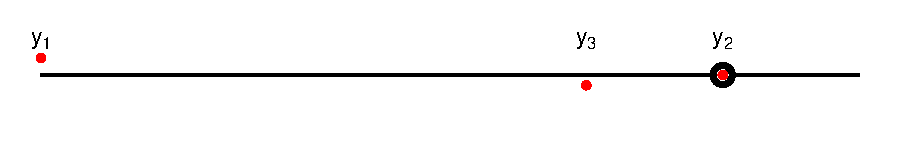
\includegraphics[width=.8\textwidth]{figure/bus_going_backwards-1} 

}

\caption[Visual demonstration of the ``reversing bus'' phenomenon]{Three sequential observations of a vehicle approaching an intersection (hollow circle). When the bus nears the intersection, it reports its position exactly at the intersection ($\Vobs_2$); however, there is a queue at this intersection, so the next observation ($\Vobs_3$) is behind the previous one, demonstrating the ``reversing bus'' phenomenon.}\label{fig:bus_going_backwards}
\end{figure}


\end{knitrout}


The effect this has on the \pf{} is that, after observing $\Vobs_2$, the vehicle's state (represented by a sample of particles) will all be around the intersection. On receiving the next observation $\Vobs_3$, the particles are transitioned \emph{forward} by $(\Vtime_3 - \Vtime_2)$~seconds, which places them at or beyond the intersection; none of the particles will be near observation $\Vobs_3$ and will likely all have a likelihood of zero. In this case, the particle filter has degenerated and needs reinitialising.


A similar situation occurs when approaching a bus stop that has an intersection just before it. Here, the bus gets stopped at the intersection, but not before reporting its position at the stop since it was almost there. A subsequent observation then shows the bus at the intersection, which again appears to involve a reversing bus. The main issue we face is that \emph{we do not know the location of intersections} since there is no easily accessible data for this.\footnote{We presented an intersection model, but this was more of a demonstration of flexibility, not of functionality.}


Checking for the bus-reversing scenario in real-time requires mapping of observations onto the route shape; that is, the \emph{inverse measurement function}, allowing us to detect if the bus has gone backwards:
\begin{equation}
\label{eq:vehicle_rev_check}
\Vmeas^{-1}(\Vobs_k) < \Vmeas^{-1}(\Vobs_{k-1}).
\end{equation}
Of course, the inverse function is not exact, since the true location is unlikely to be positioned exactly on the line (roads have width, and \gls{gps} devices have error). To compute $\Vmeas^{-1}$, we find the shortest distance along the route's shape that is closer than a threshold of $3\GPSerr$, which allows for situations where the route passes the observed location point more than once (such as in loops).

If the observation is determined to be going backwards, we have to decide between
\begin{enumerate}[i.]
\item ignoring the current observation, or
\item ignoring the previous observation and restoring the vehicle's previous state.
\end{enumerate}
If we can determine that the first observation is a pre-emptive observation (that is, at a waypoint), then option (ii) is the logical choice, although this requires storing each vehicle's state \emph{twice}. Otherwise, it is easier to ignore the current observation completely and use option (i). Note that, were intersection locations knowable, we could include this behaviour in the model; as it stands, however, this workaround is required to avoid unnecessary degeneration.


\paragraph{Buses that remain stationary}

Another situation (which can also occur around unknown intersections) is when the bus does not move between successive observations (or it moves very slowly). For example, the bus may need to turn onto a major road, for which there is a queue of traffic. The bus will report its position when it arrives, and may again report its position after moving a few meters. If our model does not allow for the bus to suddenly slow down in these situations, the particles will all be far ahead of the bus and degeneration will occur.


We can determine if the bus has remained more-or-less stationary by computing the distance between successive observations and comparing to a threshold:
\begin{equation}
\label{eq:vehicle_dist_check}
\dist{\Vobs_{k-1}, \Vobs_k} < \distThreshold =
\Vtdiff_k \min_i\left(\Vspeed_k\vi\right).
\end{equation}
The threshold here is the expected distance travelled in $\Vtdiff_k$~seconds by the slowest particle. Rather than slowing the particles (which could run into the opposite problem once the vehicle passes through the intersection), we sample a temporary speed,
\begin{equation}
\label{eq:vehicle_temp_speed}
\Vspeed_k\vi \sim
\Uniform{0}{\frac{\dist{\Vobs_{k-1}, \Vobs_k}}{\Vtdiff_k}},
\end{equation}
which is used for one single iteration.

Again, if we knew the locations of intersections, we could integrate this behaviour into the model. Particles could partake in ``creeping'' up to the intersection, before quickly accelerating back up to speed on the next road segment. Even then, however, the above behaviour would still need to be included to handle non-intersection related slowing down, for example, when reaching a congested section of a road.

\subsection{Parameter selection}
\label{sec:pf_params}

Once the inherent data issues have been dealt with,
we can begin determining the values of the model parameters.
Some of these are fixed and constant across all vehicles, routes, and stops,
for example,
GPS error, $\GPSerr$,
system noise, $\Vnoise$,
and minimum dwell time, $\mindwell$.
Others will inevitably vary between routes, stops, and time of day,
such as stopping probability, $\Prstop$,
and dwell time, $\dwell$.


% We explore these by modelling a subset of routes throughout Auckland over several days,
% using historical data to allow us to vary parameters and compare their effects.
% Some parameters, notably $\GPSerr$ and $\dwell$
% can be determined from the data:
% the value $\GPSerr$ can be approximated by looking at the variability
% of points around the route,
% since we assume there is no directional bias,
% so the distance from an observation to the route is an approximate estimate
% of measurement error.


\subsubsection{GPS error}
\label{sec:pf_params_gps}

The GPS or \emph{measurement} error used in the model has a strong effect on performance, as we saw in \cref{sec:pf_issues}. We can get a simple estimate of GPS error by examining the distribution of observations around the route; that is, we computed the shortest distance between the route and each observation, and graphed the results in \cref{fig:pf_param_gps}. We see two modes at about 0.5 and 2.5~meters, which could be due to a multitude of reasons. One likely one, however, is \emph{road width}, since the route shapes typically run in the middle of the road and the buses drive either side of the center line. Single-lane roads will have a smaller average distance between the bus and the center line, while for roads with two or more lanes, this will be larger. Additionally, some roads have a median (either painted or raised) which further increases the distance between the bus and the ``center line''. It is possible that some combination of this could result in the distribution shown in \cref{fig:pf_param_gps}.



\begin{knitrout}\small
\definecolor{shadecolor}{rgb}{0.969, 0.969, 0.969}\color{fgcolor}\begin{figure}
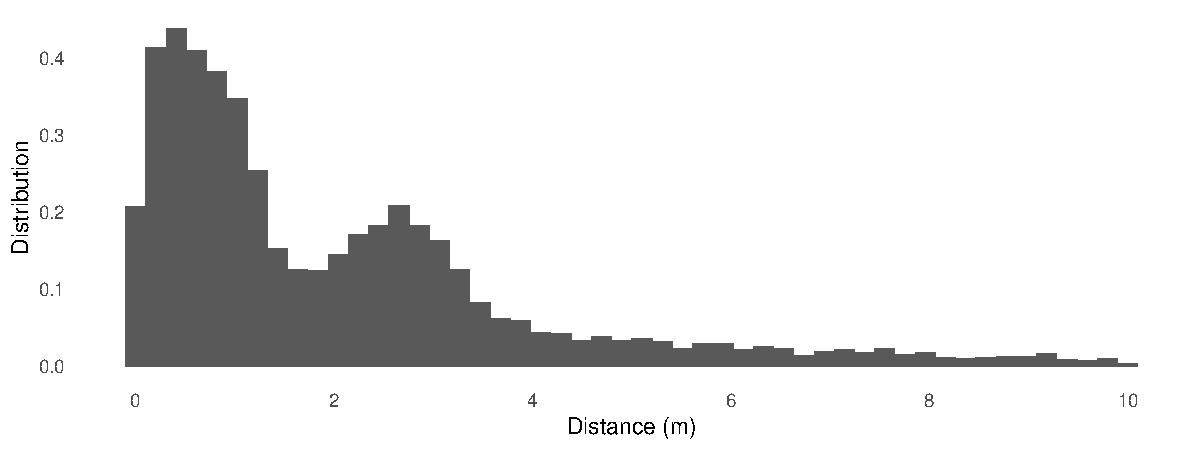
\includegraphics[width=\maxwidth]{figure/pf_param_gps-1} \caption[Distribution of distance from observation to nearest point on the route, truncated to 10~m]{Distribution of distance from observation to nearest point on the route, truncated to 10~m.}\label{fig:pf_param_gps}
\end{figure}


\end{knitrout}

The other issue is the heavy tail in the distribution of distance to path, which we trunctated to 10~meters to more easily see the modes. GPS devices usually have good accuracy, but occasionally they may be quite far off of the true location, possibly due to physical interference. 6\% of bus observations were more than 10~meters from the shape, excluding any observations greater than 50~meters since these were most likely attributed to the wrong trip (and therefore not anywhere near the route path). This would explain a large proportion of the degeneration rate (\cref{fig:model_performance_degen}), which we saw previously decreases significantly with increased GPS error.





\subsubsection{System noise}
\label{sec:pf_params_noise}

The definition of system noise is model-dependent; for transition models $f_{A1}$ and $f_{A2}$ it is \emph{the average change in speed per second}, while for model $f_{A3}$ it is \emph{the average change in acceleration per second}. From the simulations in \cref{sec:pf_issues}, we demonstrated that system noise affected the performance of the particle filter (how often resampling is required) but neither the degeneration rate nor parameter estimation.

Unlike GPS error, it is not possible to estimate system noise directly from the data. Indeed, most of the time a vehicle's speed is constant, but may change suddenly at certain locations (which are unknown), so the system noise must allow for this. We found that a smaller value of system noise under the second transition model $f_{A2}$ gave the best results in terms of sampling possible trajectories, and as such this was the model used during the simulation.



\subsubsection{Dwell times}
\label{sec:pf_params_dwell}

We are able to observe a large proportion of dwell times at stops, by compiling all those for which we have observed both arrival times $\Varr_{srm}$ and departure times $\Vdep_{srm}$ at stop $m$ of trip $r$ on day $s$ giving us a set of dwell times
\begin{equation}
\label{eq:dwell_time_obs}
\Vdwell_{srm} = \Vdep_{srm} - \Varr_{srm}
\end{equation}

\begin{knitrout}\small
\definecolor{shadecolor}{rgb}{0.969, 0.969, 0.969}\color{fgcolor}\begin{figure}
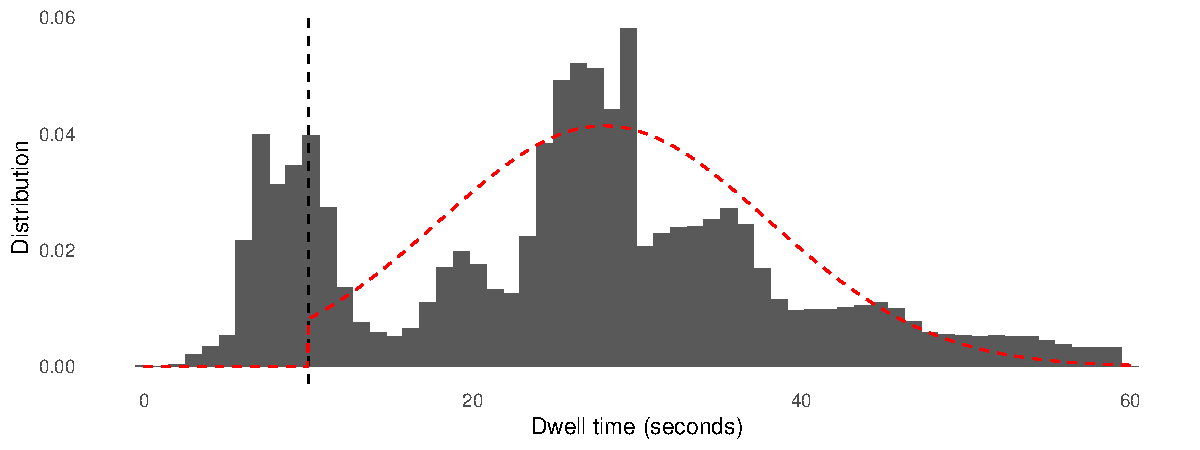
\includegraphics[width=\maxwidth]{figure/observed_dwell-1} \caption[Distribution of dwell times observed over the course of five days, truncated at one minute]{Distribution of dwell times observed over the course of five days, truncated at one minute.}\label{fig:observed_dwell}
\end{figure}


\end{knitrout}

There is no precise way to measure the minimum dwell time parameter $mindwell$. \cite{Hans_2015} used $\mindwell = 6$~seconds, which is marked by a dashed vertical line in \cref{fig:observed_dwell}. There are a few dwell times less than this, but given the spike at 6~seconds, it seems reasonable to continue with this value.

The raw data from five~days' observations are shown in \cref{fig:observed_dwell}. Here, we see an interesting pattern with apparent peaks every nine~seconds. While we could not determine the precise cause, we assume it to be due to a systematic problem in the arrival time recording system used to collect the data. From the historical dwell time data, we were able to estimate the mean and variance of dwell time for each stop $j$, $\bar\dwell_j$ and $\dwellvar_j$, respectively, which could then be used in the dwell time model.


The dwell times for each stop calcualted above \emph{include} the minimum dwell time phase. To avoid having to recompute each stop's dwell time parameter whenever $\mindwell$ is changed, we adjusted the mean of each stop's dwell time at run time to account for the minimum dwell time. That is, we use $\dwell_j = \bar\dwell_j - \mindwell$ in \cref{eq:stop_dwell_time}.


